% Options for packages loaded elsewhere
\PassOptionsToPackage{unicode}{hyperref}
\PassOptionsToPackage{hyphens}{url}
\PassOptionsToPackage{dvipsnames,svgnames,x11names}{xcolor}
\documentclass[
  12pt,
  a4paper,
]{article}
\usepackage{xcolor}
\usepackage[top=2.5cm,bottom=2.5cm,left=3cm,right=2cm]{geometry}
\usepackage{amsmath,amssymb}
\setcounter{secnumdepth}{5}
\usepackage{iftex}
\ifPDFTeX
  \usepackage[T1]{fontenc}
  \usepackage[utf8]{inputenc}
  \usepackage{textcomp} % provide euro and other symbols
\else % if luatex or xetex
  \usepackage{unicode-math} % this also loads fontspec
  \defaultfontfeatures{Scale=MatchLowercase}
  \defaultfontfeatures[\rmfamily]{Ligatures=TeX,Scale=1}
\fi
\usepackage{lmodern}
\ifPDFTeX\else
  % xetex/luatex font selection
    \setmainfont[]{Times New Roman}
    \setmonofont[Scale=0.85]{Liberation Mono}
\fi
% Use upquote if available, for straight quotes in verbatim environments
\IfFileExists{upquote.sty}{\usepackage{upquote}}{}
\IfFileExists{microtype.sty}{% use microtype if available
  \usepackage[]{microtype}
  \UseMicrotypeSet[protrusion]{basicmath} % disable protrusion for tt fonts
}{}
\makeatletter
\@ifundefined{KOMAClassName}{% if non-KOMA class
  \IfFileExists{parskip.sty}{%
    \usepackage{parskip}
  }{% else
    \setlength{\parindent}{0pt}
    \setlength{\parskip}{6pt plus 2pt minus 1pt}}
}{% if KOMA class
  \KOMAoptions{parskip=half}}
\makeatother
\usepackage{color}
\usepackage{fancyvrb}
\newcommand{\VerbBar}{|}
\newcommand{\VERB}{\Verb[commandchars=\\\{\}]}
\DefineVerbatimEnvironment{Highlighting}{Verbatim}{commandchars=\\\{\}}
% Add ',fontsize=\small' for more characters per line
\newenvironment{Shaded}{}{}
\newcommand{\AlertTok}[1]{\textcolor[rgb]{1.00,0.00,0.00}{\textbf{#1}}}
\newcommand{\AnnotationTok}[1]{\textcolor[rgb]{0.38,0.63,0.69}{\textbf{\textit{#1}}}}
\newcommand{\AttributeTok}[1]{\textcolor[rgb]{0.49,0.56,0.16}{#1}}
\newcommand{\BaseNTok}[1]{\textcolor[rgb]{0.25,0.63,0.44}{#1}}
\newcommand{\BuiltInTok}[1]{\textcolor[rgb]{0.00,0.50,0.00}{#1}}
\newcommand{\CharTok}[1]{\textcolor[rgb]{0.25,0.44,0.63}{#1}}
\newcommand{\CommentTok}[1]{\textcolor[rgb]{0.38,0.63,0.69}{\textit{#1}}}
\newcommand{\CommentVarTok}[1]{\textcolor[rgb]{0.38,0.63,0.69}{\textbf{\textit{#1}}}}
\newcommand{\ConstantTok}[1]{\textcolor[rgb]{0.53,0.00,0.00}{#1}}
\newcommand{\ControlFlowTok}[1]{\textcolor[rgb]{0.00,0.44,0.13}{\textbf{#1}}}
\newcommand{\DataTypeTok}[1]{\textcolor[rgb]{0.56,0.13,0.00}{#1}}
\newcommand{\DecValTok}[1]{\textcolor[rgb]{0.25,0.63,0.44}{#1}}
\newcommand{\DocumentationTok}[1]{\textcolor[rgb]{0.73,0.13,0.13}{\textit{#1}}}
\newcommand{\ErrorTok}[1]{\textcolor[rgb]{1.00,0.00,0.00}{\textbf{#1}}}
\newcommand{\ExtensionTok}[1]{#1}
\newcommand{\FloatTok}[1]{\textcolor[rgb]{0.25,0.63,0.44}{#1}}
\newcommand{\FunctionTok}[1]{\textcolor[rgb]{0.02,0.16,0.49}{#1}}
\newcommand{\ImportTok}[1]{\textcolor[rgb]{0.00,0.50,0.00}{\textbf{#1}}}
\newcommand{\InformationTok}[1]{\textcolor[rgb]{0.38,0.63,0.69}{\textbf{\textit{#1}}}}
\newcommand{\KeywordTok}[1]{\textcolor[rgb]{0.00,0.44,0.13}{\textbf{#1}}}
\newcommand{\NormalTok}[1]{#1}
\newcommand{\OperatorTok}[1]{\textcolor[rgb]{0.40,0.40,0.40}{#1}}
\newcommand{\OtherTok}[1]{\textcolor[rgb]{0.00,0.44,0.13}{#1}}
\newcommand{\PreprocessorTok}[1]{\textcolor[rgb]{0.74,0.48,0.00}{#1}}
\newcommand{\RegionMarkerTok}[1]{#1}
\newcommand{\SpecialCharTok}[1]{\textcolor[rgb]{0.25,0.44,0.63}{#1}}
\newcommand{\SpecialStringTok}[1]{\textcolor[rgb]{0.73,0.40,0.53}{#1}}
\newcommand{\StringTok}[1]{\textcolor[rgb]{0.25,0.44,0.63}{#1}}
\newcommand{\VariableTok}[1]{\textcolor[rgb]{0.10,0.09,0.49}{#1}}
\newcommand{\VerbatimStringTok}[1]{\textcolor[rgb]{0.25,0.44,0.63}{#1}}
\newcommand{\WarningTok}[1]{\textcolor[rgb]{0.38,0.63,0.69}{\textbf{\textit{#1}}}}
\usepackage{longtable,booktabs,array}
\usepackage{calc} % for calculating minipage widths
% Correct order of tables after \paragraph or \subparagraph
\usepackage{etoolbox}
\makeatletter
\patchcmd\longtable{\par}{\if@noskipsec\mbox{}\fi\par}{}{}
\makeatother
% Allow footnotes in longtable head/foot
\IfFileExists{footnotehyper.sty}{\usepackage{footnotehyper}}{\usepackage{footnote}}
\makesavenoteenv{longtable}
\usepackage{graphicx}
\makeatletter
\newsavebox\pandoc@box
\newcommand*\pandocbounded[1]{% scales image to fit in text height/width
  \sbox\pandoc@box{#1}%
  \Gscale@div\@tempa{\textheight}{\dimexpr\ht\pandoc@box+\dp\pandoc@box\relax}%
  \Gscale@div\@tempb{\linewidth}{\wd\pandoc@box}%
  \ifdim\@tempb\p@<\@tempa\p@\let\@tempa\@tempb\fi% select the smaller of both
  \ifdim\@tempa\p@<\p@\scalebox{\@tempa}{\usebox\pandoc@box}%
  \else\usebox{\pandoc@box}%
  \fi%
}
% Set default figure placement to htbp
\def\fps@figure{htbp}
\makeatother
\ifLuaTeX
\usepackage[bidi=basic]{babel}
\else
\usepackage[bidi=default]{babel}
\fi
\babelprovide[main,import]{vietnamese}
\ifPDFTeX
\else
\babelfont{rm}[]{Times New Roman}
\fi
% get rid of language-specific shorthands (see #6817):
\let\LanguageShortHands\languageshorthands
\def\languageshorthands#1{}
\setlength{\emergencystretch}{3em} % prevent overfull lines
\providecommand{\tightlist}{%
  \setlength{\itemsep}{0pt}\setlength{\parskip}{0pt}}
\usepackage{fvextra}
\DefineVerbatimEnvironment{Highlighting}{Verbatim}{breaklines,breakanywhere,commandchars=\\\{\}}
\fvset{breaklines,breakanywhere}
\usepackage{float}
\floatplacement{figure}{H}
\usepackage[font=small,labelfont=bf,labelsep=period]{caption}
\usepackage{setspace}
\setstretch{1.2}
\usepackage{fancyhdr}
\pagestyle{fancy}
\fancyhf{}
\fancyhead[L]{\small\nouppercase{\leftmark}}
\fancyhead[R]{\small Báo cáo thực hành Xử lý dữ liệu lớn}
\fancyfoot[C]{\small\thepage}
\renewcommand{\headrulewidth}{0.4pt}
\AtBeginDocument{%
  \renewcommand{\figurename}{Hình}%
  \renewcommand{\tablename}{Bảng}%
  \renewcommand{\contentsname}{Mục lục}%
  \renewcommand{\listfigurename}{Danh mục hình}%
  \renewcommand{\listtablename}{Danh mục bảng}%
  \providecommand{\chaptername}{}\renewcommand{\chaptername}{Chương}%
}
% Symbols missing from Times New Roman: typeset them in math mode instead.
\begingroup
\catcode`⌈=\active \catcode`⌉=\active \catcode`≫=\active \catcode`≪=\active
\protected\gdef⌈{\ensuremath{\lceil}}\protected\gdef⌉{\ensuremath{\rceil}}
\protected\gdef≫{\ensuremath{\gg}}\protected\gdef≪{\ensuremath{\ll}}
\endgroup
\AtBeginDocument{\catcode`⌈=\active \catcode`⌉=\active \catcode`≫=\active \catcode`≪=\active}
\usepackage{bookmark}
\IfFileExists{xurl.sty}{\usepackage{xurl}}{} % add URL line breaks if available
\urlstyle{same}
\hypersetup{
  pdflang={vi},
  colorlinks=true,
  linkcolor={black},
  filecolor={Maroon},
  citecolor={Blue},
  urlcolor={blue},
  pdfcreator={LaTeX via pandoc}}

\author{}
\date{}

\begin{document}

\begin{titlepage}
\centering
{\large\MakeUppercase{Trường Đại học Khoa học Tự nhiên, ĐHQG-HCM}\par}
{\large\bfseries\MakeUppercase{Khoa Toán - Tin học}\par}
\vspace{0.4cm}\rule{0.55\textwidth}{0.6pt}\par
\vspace{1.2cm}
\includegraphics[width=4.5cm]{/data/logo-hcmus.png}\par
\vspace{1.2cm}
{\Large\bfseries BÁO CÁO THỰC HÀNH\par}
\vspace{0.3cm}
{\large Môn học: Xử lý dữ liệu lớn\par}
\vspace{1.5cm}
{\large\bfseries Bài thực hành L04\par}
\vspace{0.4cm}
{\LARGE\bfseries Nạp dữ liệu từ cơ sở dữ liệu OLTP vào HDFS: Sqoop và
Spark JDBC, nạp toàn phần và nạp gia tăng\par}
\vfill
\begin{tabular}{@{}ll@{}}
Sinh viên thực hiện:  & Nguyễn Thị Huyền Trang \\[2pt]
Mã số sinh viên:      & 23280092 \\[2pt]
Lớp:                  & 23KDL \\
\end{tabular}
\vfill
{\large TP. Hồ Chí Minh, Tháng 10 năm 2026\par}
\end{titlepage}

{
\hypersetup{linkcolor=black}
\setcounter{tocdepth}{3}
\tableofcontents
}
\listoffigures
\listoftables
\section{Mục tiêu và môi trường}\label{sec:l04-intro}

Bài thực hành nạp dữ liệu từ PostgreSQL vào HDFS bằng Apache Sqoop 1.4.7
(đã vào Apache Attic từ tháng 6 năm 2021) {[}1{]} và Spark JDBC {[}2{]},
theo hai cách nạp toàn phần và nạp gia tăng, rồi so sánh hai công cụ.
PostgreSQL chạy với
\texttt{log\_}\allowbreak{}\texttt{statement=}\allowbreak{}\texttt{all}\allowbreak{}
để đọc trực tiếp câu SQL mà mỗi công cụ gửi xuống. Hệ thống chạy bằng
Docker Compose trên một máy (Bảng~\ref{tbl:l04-env}). Container
\texttt{jdbc-driver} chỉ tải driver rồi thoát với mã 0; ban đầu chúng
tôi tưởng nó lỗi, nhưng đó là hành vi đúng (Hình~\ref{fig:l04-stack}).

\begin{longtable}[]{@{}
  >{\raggedright\arraybackslash}p{(\linewidth - 2\tabcolsep) * \real{0.5000}}
  >{\raggedright\arraybackslash}p{(\linewidth - 2\tabcolsep) * \real{0.5000}}@{}}
\caption{\label{tbl:l04-env}Môi trường thực nghiệm (stack
\texttt{l04\_ingestion}).}\tabularnewline
\toprule\noalign{}
\begin{minipage}[b]{\linewidth}\raggedright
Thành phần
\end{minipage} & \begin{minipage}[b]{\linewidth}\raggedright
Phiên bản / cấu hình
\end{minipage} \\
\midrule\noalign{}
\endfirsthead
\toprule\noalign{}
\begin{minipage}[b]{\linewidth}\raggedright
Thành phần
\end{minipage} & \begin{minipage}[b]{\linewidth}\raggedright
Phiên bản / cấu hình
\end{minipage} \\
\midrule\noalign{}
\endhead
\bottomrule\noalign{}
\endlastfoot
PostgreSQL & 18.6,
\texttt{log\_}\allowbreak{}\texttt{statement=}\allowbreak{}\texttt{all}\allowbreak{},
cơ sở dữ liệu nguồn Olist \\
HDFS & 3.4.3, 1 NameNode + 1 DataNode \\
YARN & ResourceManager, NodeManager, JobHistory Server (chạy job của
Sqoop) \\
Sqoop & 1.4.7 (image khóa học
\texttt{de-labs/}\allowbreak{}\texttt{sqoop:}\allowbreak{}\texttt{1.}\allowbreak{}\texttt{4.}\allowbreak{}\texttt{7}\allowbreak{}) \\
Spark & 4.1.3, local mode, Spark UI cổng 4040 \\
JDBC driver & PostgreSQL JDBC
(\texttt{/}\allowbreak{}\texttt{jars/}\allowbreak{}\texttt{postgresql.}\allowbreak{}\texttt{jar}\allowbreak{}),
dùng chung cho Sqoop và Spark \\
\end{longtable}

\begin{figure}
\centering
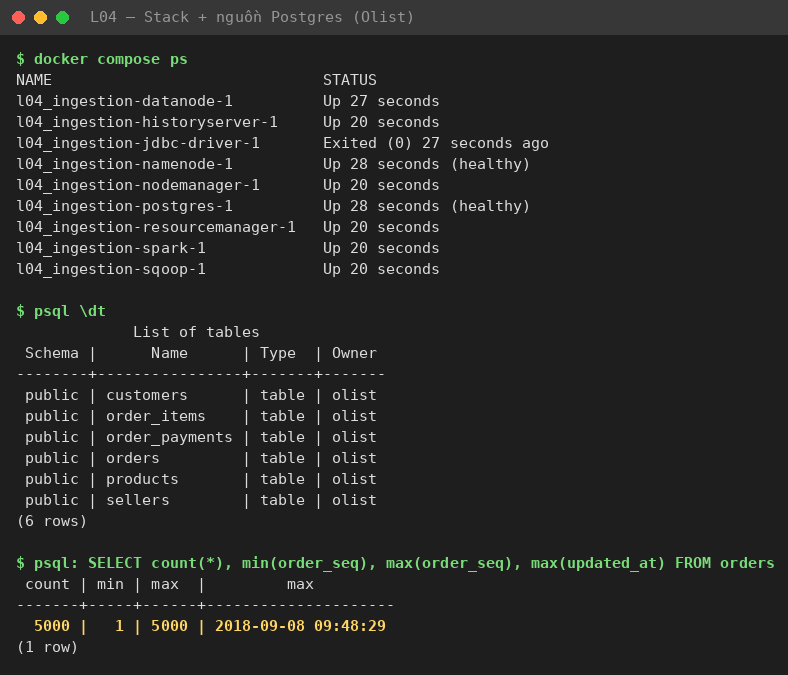
\includegraphics[width=0.85\linewidth,height=\textheight,keepaspectratio]{img/01_stack_and_source.png}
\caption{Trạng thái container của stack L04 và 6 bảng nguồn trong
PostgreSQL.}\label{fig:l04-stack}
\end{figure}

Nguồn là cơ sở dữ liệu Olist tổng hợp gồm 6 bảng (\texttt{customers},
\texttt{orders}, \texttt{order\_items}, \texttt{order\_payments},
\texttt{products}, \texttt{sellers}). Bảng \texttt{orders} có 5,000
dòng, \texttt{order\_seq} chạy từ 1 đến 5000, \texttt{max(updated\_at)}
là
\texttt{2018-09-08\ 09:}\allowbreak{}\texttt{48:}\allowbreak{}\texttt{29}\allowbreak{}.
\texttt{order\_seq} là khóa thay thế kiểu số, tăng theo thời gian mua,
còn \texttt{order\_id}, \texttt{customer\_id} là chuỗi hash 32 ký tự.
Mỗi bảng có cột \texttt{updated\_at} do trigger tự cập nhật khi UPDATE.
Phân bố trạng thái đơn hàng lấy bằng \texttt{sqoop\ eval} nằm ở
Bảng~\ref{tbl:l04-status}.

\begin{longtable}[]{@{}ll@{}}
\caption{\label{tbl:l04-status}Phân bố trạng thái của 5,000 đơn hàng ban
đầu.}\tabularnewline
\toprule\noalign{}
\texttt{order\_status} & Số đơn \\
\midrule\noalign{}
\endfirsthead
\toprule\noalign{}
\texttt{order\_status} & Số đơn \\
\midrule\noalign{}
\endhead
\bottomrule\noalign{}
\endlastfoot
delivered & 4,793 \\
shipped & 102 \\
unavailable & 41 \\
canceled & 30 \\
processing & 19 \\
invoiced & 11 \\
approved & 3 \\
created & 1 \\
\end{longtable}

Script
\texttt{sql/}\allowbreak{}\texttt{simulate\_}\allowbreak{}\texttt{changes.}\allowbreak{}\texttt{sql}\allowbreak{}
chèn 3 khách hàng và 3 đơn mới, đổi 2 đơn \texttt{shipped} đầu tiên
thành \texttt{delivered}. Chúng tôi chạy nó hai lần: trước phần Sqoop
gia tăng và giữa hai lần chạy Spark gia tăng. Vì thế lúc chạy Spark,
\texttt{orders} và \texttt{customers} đã có 5,003 dòng, khác giá trị
tham chiếu trong README.

\section{Thực hiện và kết quả}\label{sec:l04-results}

\subsection{\texorpdfstring{Sqoop nạp toàn phần bảng
\texttt{orders}}{Sqoop nạp toàn phần bảng orders}}\label{sec:l04-sqoop-full}

Mỗi lệnh \texttt{import} được biên dịch thành một MapReduce job chỉ có
pha map {[}1{]}. Với
\texttt{-\/-split-by\ order\_}\allowbreak{}\texttt{seq\ -m\ 4}\allowbreak{},
Sqoop báo
\texttt{number\ of\ splits:}\allowbreak{}\texttt{4}\allowbreak{} và nhật
ký PostgreSQL có đúng 4 câu SELECT theo khoảng của 4 map
(Bảng~\ref{tbl:l04-sqoop-splits}, Hình~\ref{fig:l04-pglog-sqoop}; cách
chia giải thích ở Mục~\ref{sec:l04-q1}). Job
\texttt{job\_}\allowbreak{}\texttt{1793356967101\_}\allowbreak{}\texttt{0001}\allowbreak{}
báo
\texttt{Transferred\ 1.}\allowbreak{}\texttt{009\ MB\ in\ 25.}\allowbreak{}\texttt{2306\ seconds\ (40.}\allowbreak{}\texttt{9499\ KB/}\allowbreak{}\texttt{sec)}\allowbreak{}
và \texttt{Retrieved\ 5000\ records}\allowbreak{}; cả lệnh CLI mất 28.5
s vì còn khởi động JVM, sinh và biên dịch lớp record rồi nộp job lên
YARN.

\begin{longtable}[]{@{}llll@{}}
\caption{\label{tbl:l04-sqoop-splits}Các split của Sqoop khi nạp
\texttt{orders} với
\texttt{-\/-split-by\ order\_}\allowbreak{}\texttt{seq\ -m\ 4}\allowbreak{}.}\tabularnewline
\toprule\noalign{}
Map & Điều kiện WHERE & Số dòng & Kích thước file \\
\midrule\noalign{}
\endfirsthead
\toprule\noalign{}
Map & Điều kiện WHERE & Số dòng & Kích thước file \\
\midrule\noalign{}
\endhead
\bottomrule\noalign{}
\endlastfoot
0 &
\texttt{order\_}\allowbreak{}\texttt{seq\ \textgreater{}=}\allowbreak{}\texttt{\ 1\ AND\ order\_}\allowbreak{}\texttt{seq\ \textless{}\ 1251}\allowbreak{}
& 1,250 & 263,891 B \\
1 &
\texttt{order\_}\allowbreak{}\texttt{seq\ \textgreater{}=}\allowbreak{}\texttt{\ 1251\ AND\ order\_}\allowbreak{}\texttt{seq\ \textless{}\ 2501}\allowbreak{}
& 1,250 & 264,924 B \\
2 &
\texttt{order\_}\allowbreak{}\texttt{seq\ \textgreater{}=}\allowbreak{}\texttt{\ 2501\ AND\ order\_}\allowbreak{}\texttt{seq\ \textless{}\ 3751}\allowbreak{}
& 1,250 & 265,023 B \\
3 &
\texttt{order\_}\allowbreak{}\texttt{seq\ \textgreater{}=}\allowbreak{}\texttt{\ 3751\ AND\ order\_}\allowbreak{}\texttt{seq\ \textless{}=}\allowbreak{}\texttt{\ 5000}\allowbreak{}
& 1,250 & 264,149 B \\
\end{longtable}

Bốn file \texttt{part-m-*} gần bằng nhau cả về số dòng lẫn kích thước
(Hình~\ref{fig:l04-sqoop-full}), dạng văn bản CSV với timestamp
\texttt{2017-01-03\ 01:}\allowbreak{}\texttt{29:}\allowbreak{}\texttt{02.}\allowbreak{}\texttt{0}\allowbreak{}
và NULL ghi là \texttt{\textbackslash{}N}. JobHistory xác nhận 4 map, 0
reduce (Hình~\ref{fig:l04-jh-orders}).

\begin{figure}
\centering
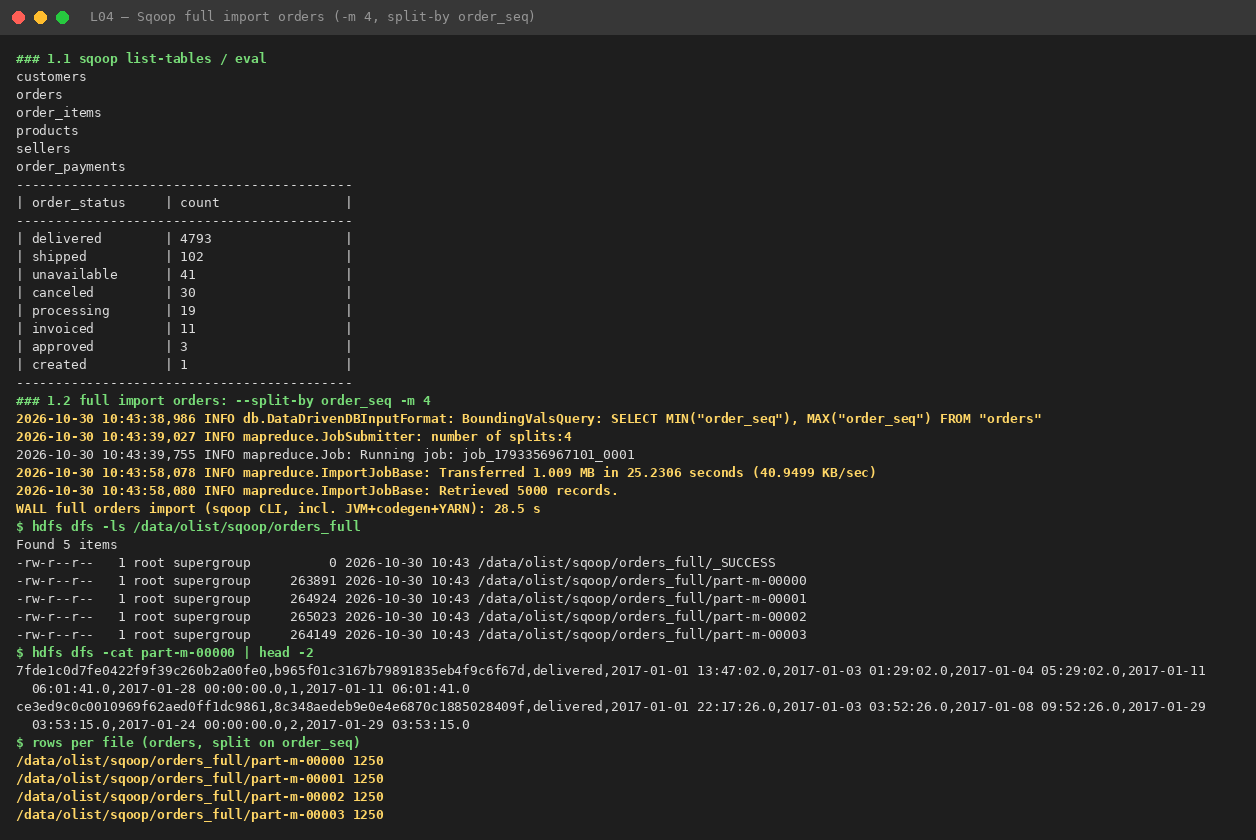
\includegraphics[width=0.85\linewidth,height=\textheight,keepaspectratio]{img/02_sqoop_full_import_orders.png}
\caption{Sqoop nạp toàn phần \texttt{orders}: bounding query, 4 split và
số dòng mỗi file.}\label{fig:l04-sqoop-full}
\end{figure}

\begin{figure}
\centering
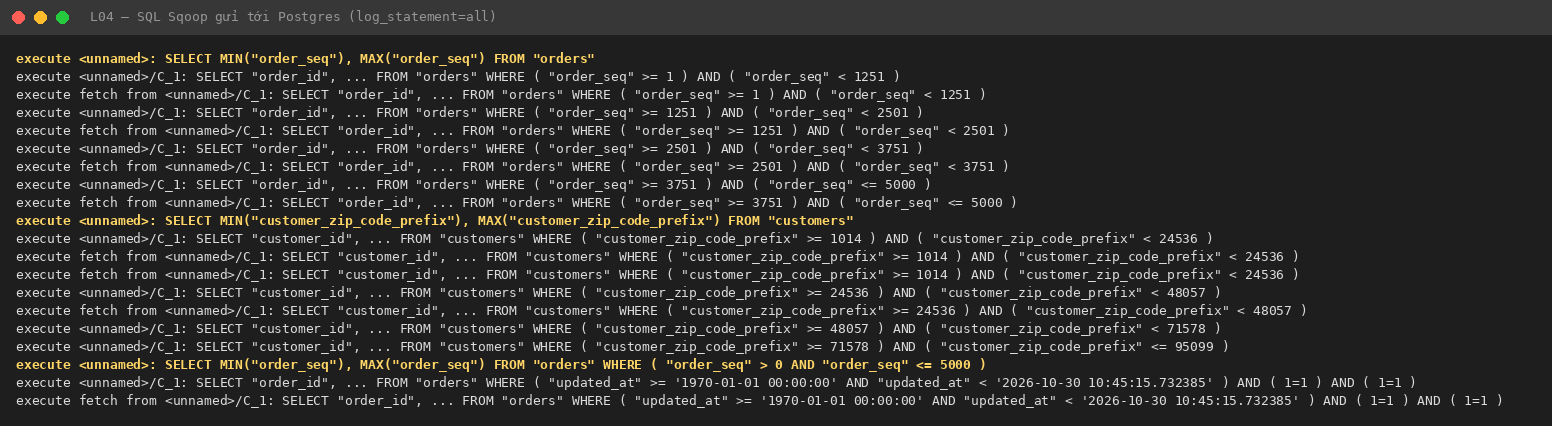
\includegraphics[width=1\linewidth,height=\textheight,keepaspectratio]{img/05_postgres_log_sqoop_sql.png}
\caption{Nhật ký PostgreSQL ghi lại bounding query và 4 câu SELECT theo
khoảng \texttt{order\_seq} do các map task của Sqoop
gửi.}\label{fig:l04-pglog-sqoop}
\end{figure}

\begin{figure}
\centering
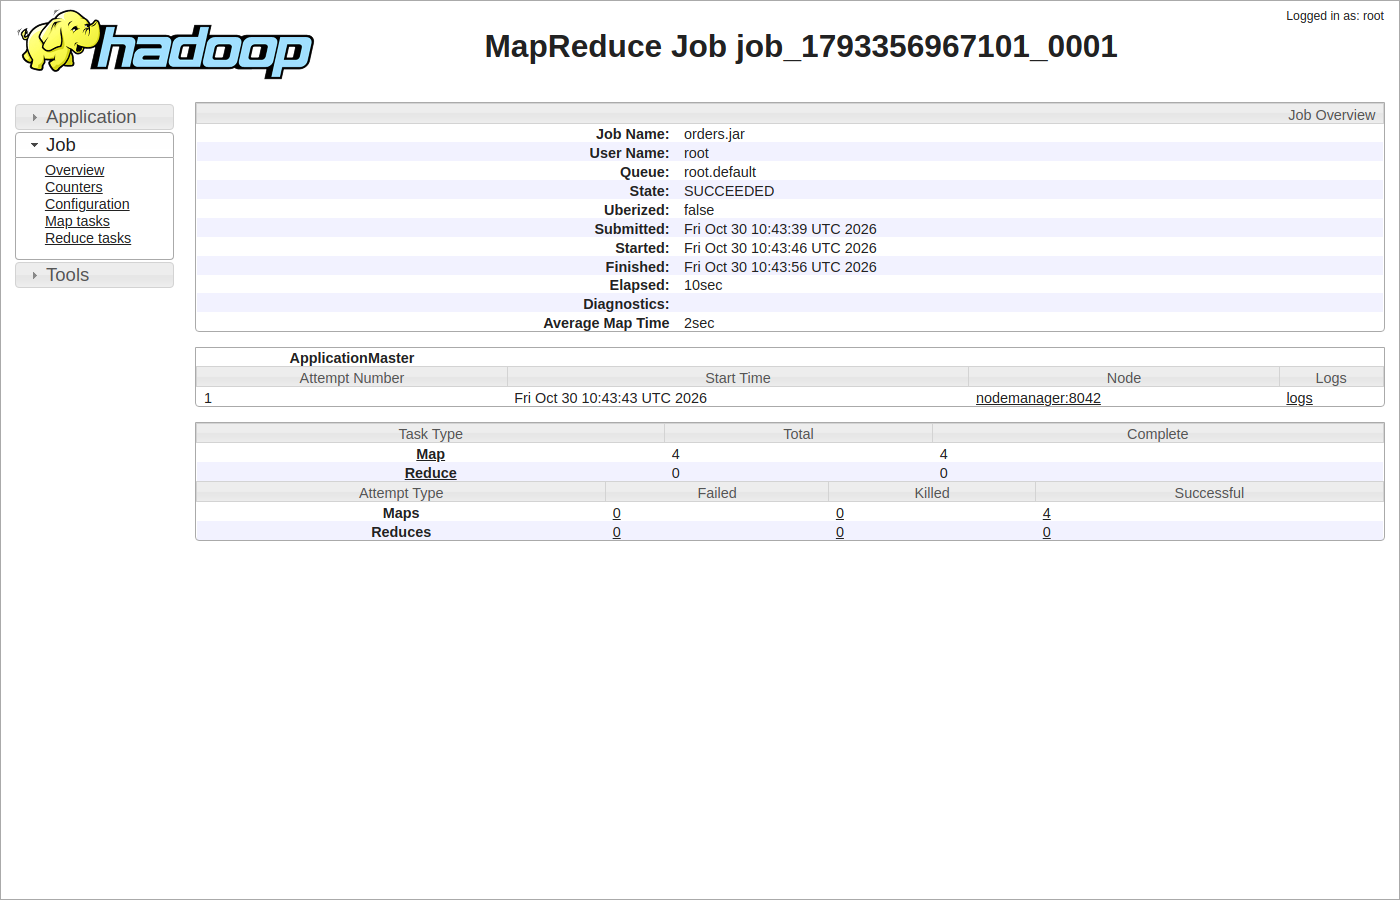
\includegraphics[width=0.85\linewidth,height=\textheight,keepaspectratio]{img/24_ui_jobhistory_orders_full_4maps.png}
\caption{JobHistory của job
\texttt{job\_}\allowbreak{}\texttt{1793356967101\_}\allowbreak{}\texttt{0001}\allowbreak{}
(\texttt{orders.jar}): 4 map task thành công, không có reduce
task.}\label{fig:l04-jh-orders}
\end{figure}

\subsection{Sqoop với cột chia bị lệch}\label{sec:l04-sqoop-skew}

Bảng \texttt{customers} được nạp với
\texttt{-\/-split-by\ customer\_}\allowbreak{}\texttt{zip\_}\allowbreak{}\texttt{code\_}\allowbreak{}\texttt{prefix\ -m\ 4}\allowbreak{}
vào
\texttt{/}\allowbreak{}\texttt{data/}\allowbreak{}\texttt{olist/}\allowbreak{}\texttt{sqoop/}\allowbreak{}\texttt{customers\_}\allowbreak{}\texttt{full}\allowbreak{}.
Bounding query trả về (1014, 95099), và nhật ký PostgreSQL cho thấy 4
khoảng rộng xấp xỉ 23,521 với các điểm cắt 24536, 48057 và 71578. Số
dòng mỗi file đặt cạnh trường hợp \texttt{orders} ở
Bảng~\ref{tbl:l04-skew}.

\begin{longtable}[]{@{}
  >{\raggedright\arraybackslash}p{(\linewidth - 8\tabcolsep) * \real{0.2000}}
  >{\raggedright\arraybackslash}p{(\linewidth - 8\tabcolsep) * \real{0.2000}}
  >{\raggedright\arraybackslash}p{(\linewidth - 8\tabcolsep) * \real{0.2000}}
  >{\raggedright\arraybackslash}p{(\linewidth - 8\tabcolsep) * \real{0.2000}}
  >{\raggedright\arraybackslash}p{(\linewidth - 8\tabcolsep) * \real{0.2000}}@{}}
\caption{\label{tbl:l04-skew}Số dòng mỗi file khi chia theo cột phân bố
đều và cột bị lệch.}\tabularnewline
\toprule\noalign{}
\begin{minipage}[b]{\linewidth}\raggedright
Bảng / cột split
\end{minipage} & \begin{minipage}[b]{\linewidth}\raggedright
part-m-00000
\end{minipage} & \begin{minipage}[b]{\linewidth}\raggedright
part-m-00001
\end{minipage} & \begin{minipage}[b]{\linewidth}\raggedright
part-m-00002
\end{minipage} & \begin{minipage}[b]{\linewidth}\raggedright
part-m-00003
\end{minipage} \\
\midrule\noalign{}
\endfirsthead
\toprule\noalign{}
\begin{minipage}[b]{\linewidth}\raggedright
Bảng / cột split
\end{minipage} & \begin{minipage}[b]{\linewidth}\raggedright
part-m-00000
\end{minipage} & \begin{minipage}[b]{\linewidth}\raggedright
part-m-00001
\end{minipage} & \begin{minipage}[b]{\linewidth}\raggedright
part-m-00002
\end{minipage} & \begin{minipage}[b]{\linewidth}\raggedright
part-m-00003
\end{minipage} \\
\midrule\noalign{}
\endhead
\bottomrule\noalign{}
\endlastfoot
\texttt{orders} / \texttt{order\_seq} (1--5000) & 1,250 & 1,250 & 1,250
& 1,250 \\
\texttt{customers} /
\texttt{customer\_}\allowbreak{}\texttt{zip\_}\allowbreak{}\texttt{code\_}\allowbreak{}\texttt{prefix}\allowbreak{}
(1014--95099) & \textbf{2,450} & 1,146 & \textbf{427} & 977 \\
\end{longtable}

Split đầu nhận gần nửa bảng, gấp khoảng 5.7 lần split thứ ba
(Hình~\ref{fig:l04-skew}). Đếm độc lập bằng \texttt{width\_bucket} trên
4 thùng (Bảng~\ref{tbl:l04-bucket}) cho cùng xu hướng: thùng chứa vùng
São Paulo (01xxx--19xxx) chiếm phần lớn khách hàng.

\begin{longtable}[]{@{}llll@{}}
\caption{\label{tbl:l04-bucket}Phân bố
\texttt{customer\_}\allowbreak{}\texttt{zip\_}\allowbreak{}\texttt{code\_}\allowbreak{}\texttt{prefix}\allowbreak{}
theo
\texttt{width\_}\allowbreak{}\texttt{bucket(.}\allowbreak{}\texttt{.}\allowbreak{}\texttt{.}\allowbreak{}\texttt{,}\allowbreak{}\texttt{\ 1003,}\allowbreak{}\texttt{\ 99990,}\allowbreak{}\texttt{\ 4)}\allowbreak{}.}\tabularnewline
\toprule\noalign{}
Thùng & min zip & max zip & Số khách hàng \\
\midrule\noalign{}
\endfirsthead
\toprule\noalign{}
Thùng & min zip & max zip & Số khách hàng \\
\midrule\noalign{}
\endhead
\bottomrule\noalign{}
\endlastfoot
1 & 1014 & 25299 & 2,603 \\
2 & 26000 & 50493 & 1,026 \\
3 & 50641 & 74897 & 552 \\
4 & 76800 & 95099 & 819 \\
\end{longtable}

\begin{figure}
\centering
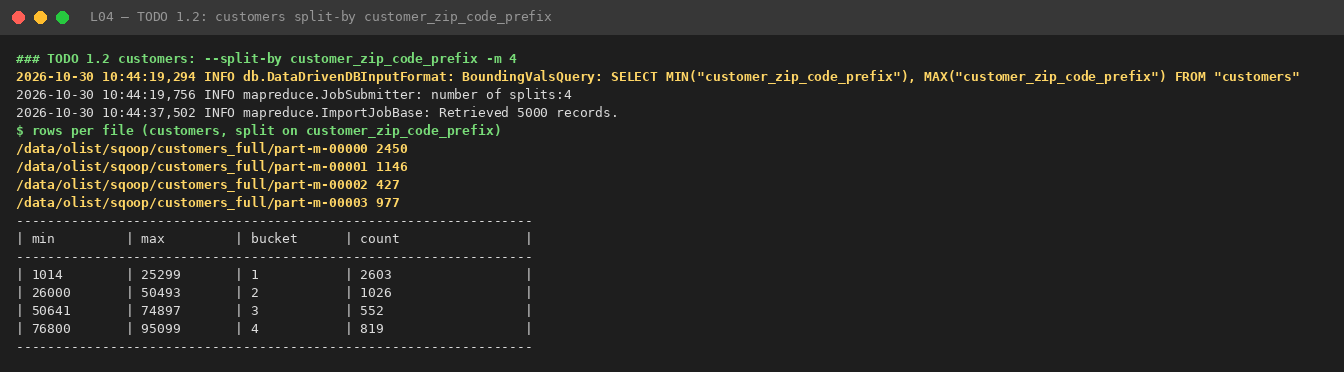
\includegraphics[width=0.85\linewidth,height=\textheight,keepaspectratio]{img/03_sqoop_customers_skew.png}
\caption{Số dòng mỗi file khi nạp \texttt{customers} chia theo
\texttt{customer\_}\allowbreak{}\texttt{zip\_}\allowbreak{}\texttt{code\_}\allowbreak{}\texttt{prefix}\allowbreak{},
thể hiện dữ liệu bị lệch.}\label{fig:l04-skew}
\end{figure}

\subsection{Sqoop nạp gia tăng, saved job, merge và
export}\label{sec:l04-sqoop-incr}

Chuỗi thao tác được tóm ở Bảng~\ref{tbl:l04-sqoop-incr}. Lần
\texttt{append} đầu (\texttt{-\/-last-value\ 0}) có điều kiện
\texttt{order\_}\allowbreak{}\texttt{seq\ \textgreater{}\ 0\ AND\ order\_}\allowbreak{}\texttt{seq\ \textless{}=}\allowbreak{}\texttt{\ 5000}\allowbreak{},
hai split \texttt{{[}1,\ 2501)} và \texttt{{[}2501,\ 5000{]}}. Saved job
\texttt{orders\_incr} lưu
\texttt{incremental.}\allowbreak{}\texttt{col\ =}\allowbreak{}\texttt{\ order\_}\allowbreak{}\texttt{seq}\allowbreak{}
và
\texttt{incremental.}\allowbreak{}\texttt{mode\ =}\allowbreak{}\texttt{\ AppendRows}\allowbreak{}
trong metastore của Sqoop.

\begin{longtable}[]{@{}
  >{\raggedright\arraybackslash}p{(\linewidth - 4\tabcolsep) * \real{0.3333}}
  >{\raggedright\arraybackslash}p{(\linewidth - 4\tabcolsep) * \real{0.3333}}
  >{\raggedright\arraybackslash}p{(\linewidth - 4\tabcolsep) * \real{0.3333}}@{}}
\caption{\label{tbl:l04-sqoop-incr}Kết quả các bước nạp gia tăng, merge
và export của Sqoop.}\tabularnewline
\toprule\noalign{}
\begin{minipage}[b]{\linewidth}\raggedright
Bước
\end{minipage} & \begin{minipage}[b]{\linewidth}\raggedright
Cửa sổ
\end{minipage} & \begin{minipage}[b]{\linewidth}\raggedright
Kết quả
\end{minipage} \\
\midrule\noalign{}
\endfirsthead
\toprule\noalign{}
\begin{minipage}[b]{\linewidth}\raggedright
Bước
\end{minipage} & \begin{minipage}[b]{\linewidth}\raggedright
Cửa sổ
\end{minipage} & \begin{minipage}[b]{\linewidth}\raggedright
Kết quả
\end{minipage} \\
\midrule\noalign{}
\endhead
\bottomrule\noalign{}
\endlastfoot
\texttt{append}, lần đầu (\texttt{-m\ 2}) & lower 0, upper 5000 & 5,000
dòng, gợi ý \texttt{-\/-last-value\ 5000}\allowbreak{} \\
\texttt{lastmodified}, cơ sở (\texttt{-m\ 1}) &
\texttt{\textquotesingle{}1970-01-01\ 00:}\allowbreak{}\texttt{00:}\allowbreak{}\texttt{00\textquotesingle{}}\allowbreak{}
đến
\texttt{\textquotesingle{}2026-10-30\ 10:}\allowbreak{}\texttt{45:}\allowbreak{}\texttt{15.}\allowbreak{}\texttt{732385\textquotesingle{}}\allowbreak{}
& 5,000 dòng \\
Saved job \texttt{orders\_incr} & &
\texttt{incremental.}\allowbreak{}\texttt{last.}\allowbreak{}\texttt{value\ =}\allowbreak{}\texttt{\ 5000}\allowbreak{} \\
\texttt{simulate\_}\allowbreak{}\texttt{changes}\allowbreak{} lần 1 & &
tạo \texttt{order\_seq} 5001--5003; đơn 139 và 278 chuyển
\texttt{delivered} \\
\texttt{sqoop\ job\ -\/-exec\ orders\_}\allowbreak{}\texttt{incr}\allowbreak{}
& lower 5000, upper 5003 & \textbf{3} dòng; \texttt{last.value} thành
5003; thư mục có 5,003 dòng \\
\texttt{lastmodified} +
\texttt{-\/-merge-key\ order\_}\allowbreak{}\texttt{id}\allowbreak{} &
\texttt{\textquotesingle{}.}\allowbreak{}\texttt{.}\allowbreak{}\texttt{.}\allowbreak{}\texttt{10:}\allowbreak{}\texttt{45:}\allowbreak{}\texttt{15.}\allowbreak{}\texttt{732385\textquotesingle{}}\allowbreak{}
đến
\texttt{\textquotesingle{}.}\allowbreak{}\texttt{.}\allowbreak{}\texttt{.}\allowbreak{}\texttt{10:}\allowbreak{}\texttt{46:}\allowbreak{}\texttt{35.}\allowbreak{}\texttt{897666\textquotesingle{}}\allowbreak{}
& \textbf{5} dòng; merge job tạo \texttt{part-r-00000} 5,003 dòng \\
\texttt{sqoop\ export} sang \texttt{orders\_copy} (\texttt{-m\ 2}) & &
1.0094 MB trong 18.4353 s, 5,000 record \\
\end{longtable}

Saved job chạy
\texttt{.}\allowbreak{}\texttt{.}\allowbreak{}\texttt{.}\allowbreak{}\texttt{\ WHERE\ (\ "order\_}\allowbreak{}\texttt{seq"\ \textgreater{}\ 5000\ AND\ "order\_}\allowbreak{}\texttt{seq"\ \textless{}=}\allowbreak{}\texttt{\ 5003\ )}\allowbreak{}
và chỉ thêm một file \texttt{part-m-00002} (420 B) cạnh hai file 528,815
B và 529,172 B của lần đầu; đơn 139 và 278 vừa cập nhật không được nạp
lại. Với \texttt{lastmodified}, do thư mục đích đã tồn tại, Sqoop chạy
thêm một merge job
(\texttt{Merged\ Map\ outputs=}\allowbreak{}\texttt{2}\allowbreak{})
thay bản cũ của cùng \texttt{order\_id} bằng bản mới. Kết quả là một
file \texttt{part-r-00000} (1,058,459 B) không trùng lặp, trong đó đơn
139 và 278 mang trạng thái \texttt{delivered} và \texttt{updated\_at}
mới. Một chi tiết chúng tôi chỉ thấy khi đọc log: \texttt{lastmodified}
dùng cửa sổ nửa mở
\texttt{updated\_}\allowbreak{}\texttt{at\ \textgreater{}=}\allowbreak{}\texttt{\ lower\ AND\ updated\_}\allowbreak{}\texttt{at\ \textless{}\ upper}\allowbreak{},
ngược với Spark ở phần sau (Hình~\ref{fig:l04-sqoop-incr},
Hình~\ref{fig:l04-sqoop-merge}).

\begin{figure}
\centering
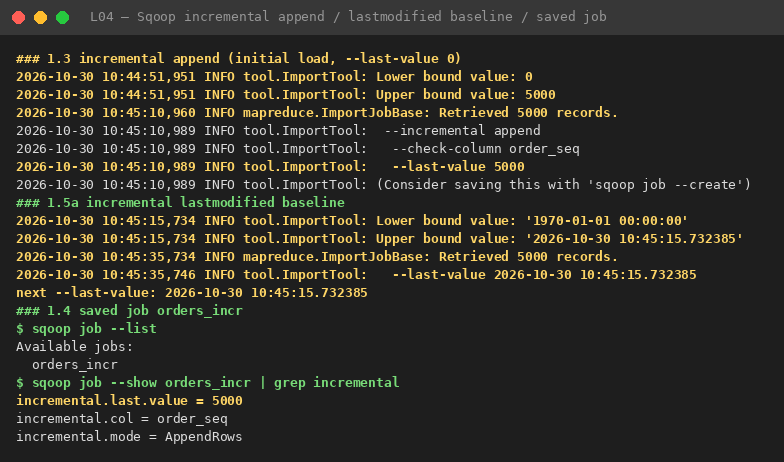
\includegraphics[width=0.85\linewidth,height=\textheight,keepaspectratio]{img/04_sqoop_incremental_and_saved_job.png}
\caption{Sqoop nạp \texttt{append} lần đầu, nạp \texttt{lastmodified} cơ
sở và tạo saved job \texttt{orders\_incr}.}\label{fig:l04-sqoop-incr}
\end{figure}

\begin{figure}
\centering
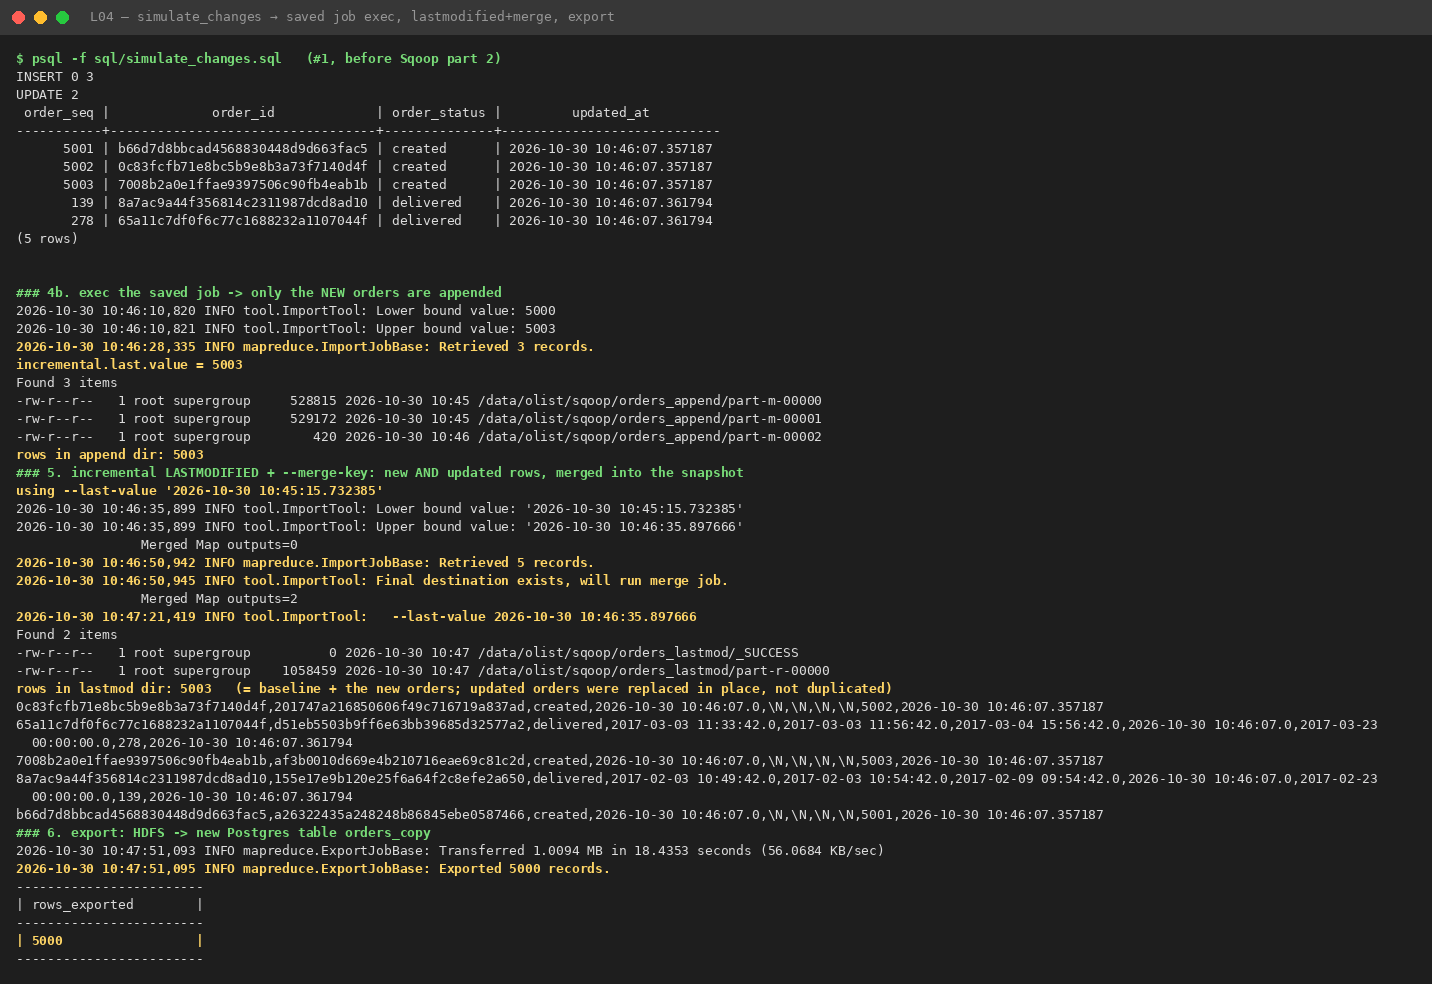
\includegraphics[width=0.85\linewidth,height=\textheight,keepaspectratio]{img/06_sqoop_after_changes_merge_export.png}
\caption{Sau
\texttt{simulate\_}\allowbreak{}\texttt{changes}\allowbreak{} lần 1:
saved job, \texttt{lastmodified} kèm merge và export về
PostgreSQL.}\label{fig:l04-sqoop-merge}
\end{figure}

ResourceManager liệt kê 8 ứng dụng MapReduce do Sqoop nộp
(\texttt{orders.jar}, \texttt{customers.jar},
\texttt{orders\_copy.jar}), đều thành công (Hình~\ref{fig:l04-yarn},
Hình~\ref{fig:l04-jh-sqoop}).

\begin{figure}
\centering
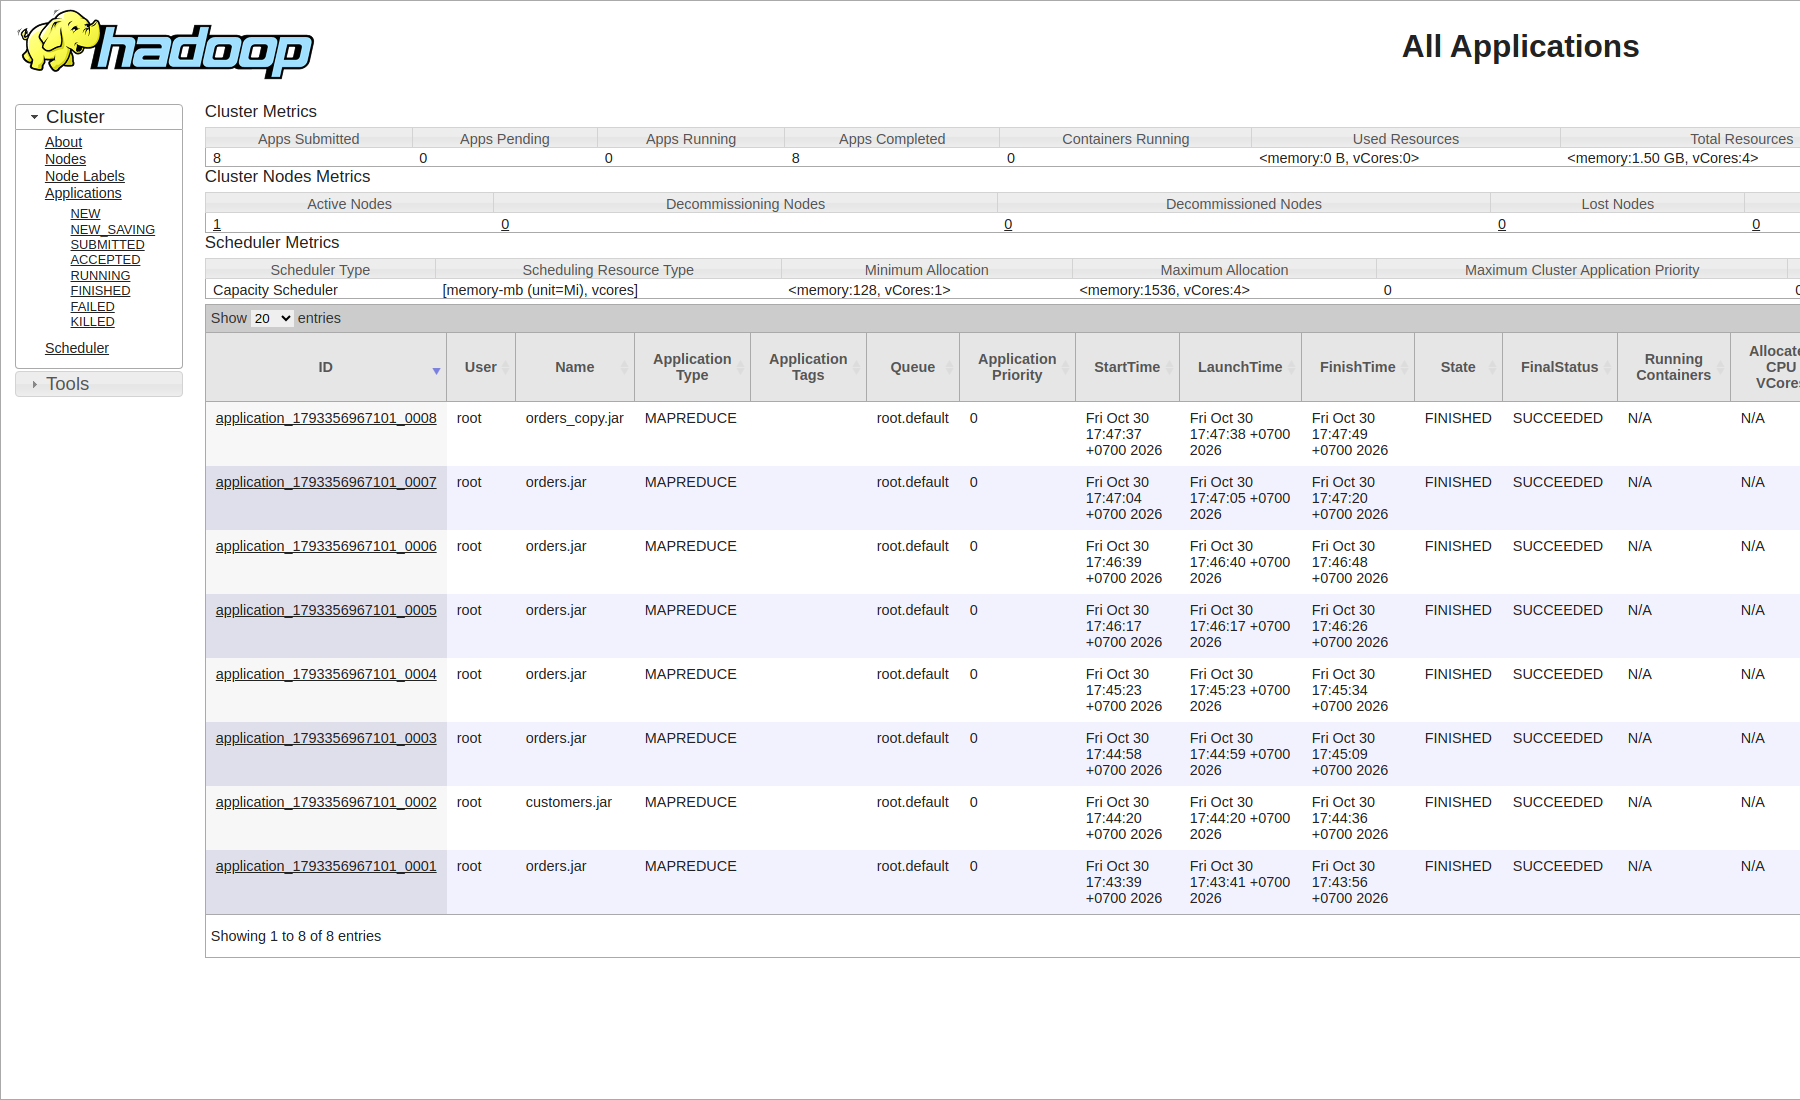
\includegraphics[width=1\linewidth,height=\textheight,keepaspectratio]{img/20_ui_yarn_sqoop_jobs.png}
\caption{YARN ResourceManager UI: các MapReduce job do Sqoop nộp, tất cả
ở trạng thái FINISHED/SUCCEEDED.}\label{fig:l04-yarn}
\end{figure}

\begin{figure}
\centering
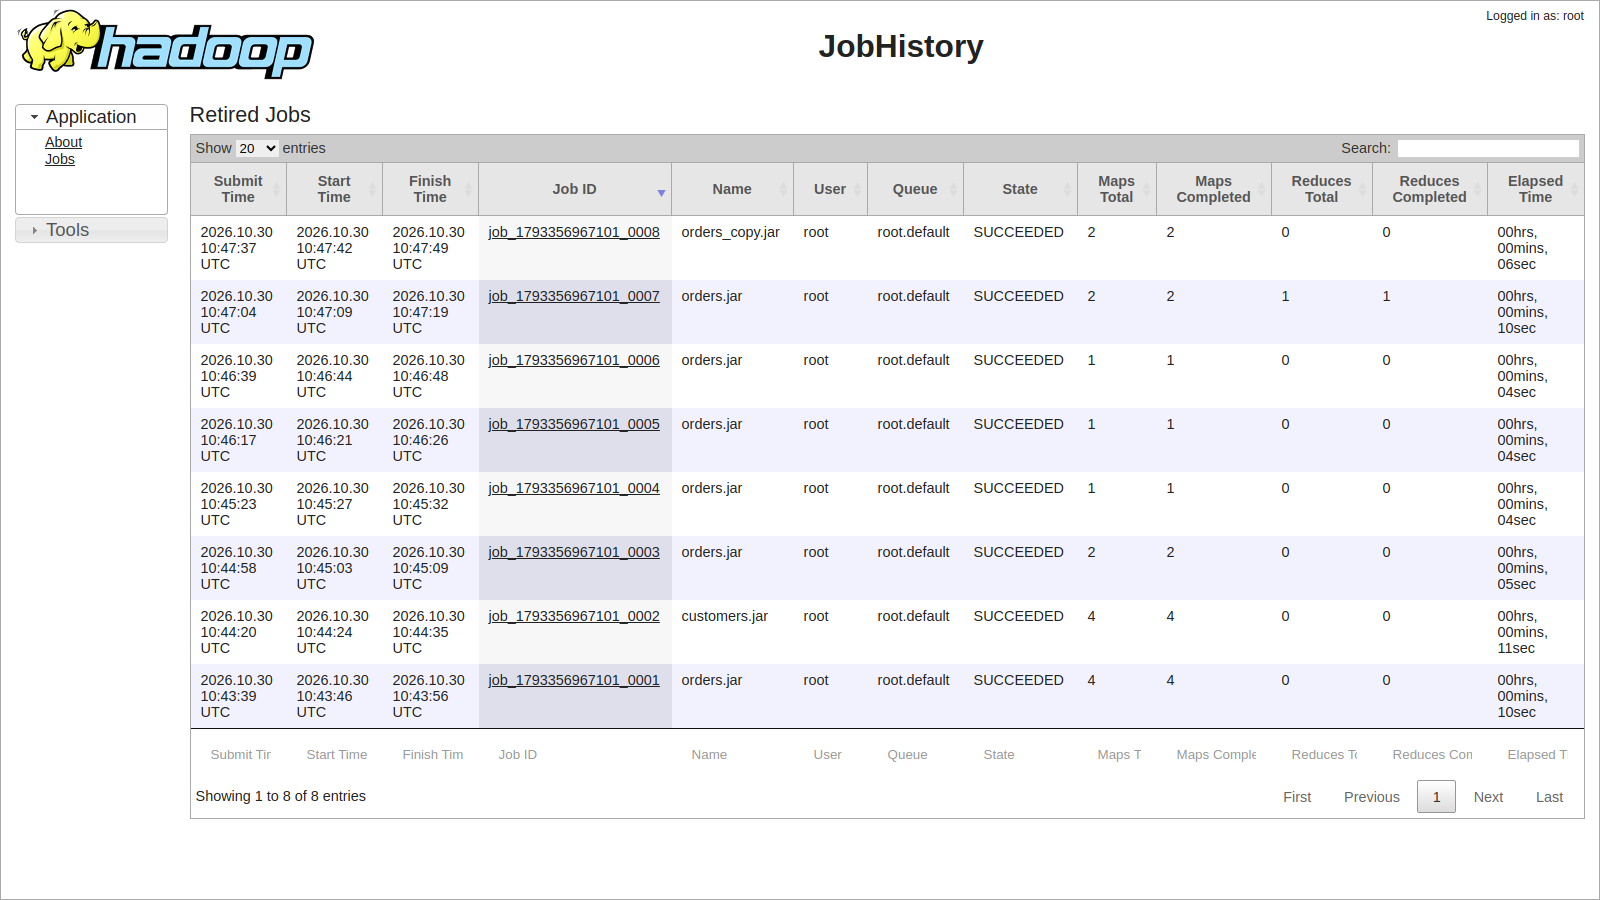
\includegraphics[width=1\linewidth,height=\textheight,keepaspectratio]{img/21_ui_jobhistory_sqoop.png}
\caption{JobHistory Server liệt kê các job Sqoop đã hoàn
tất.}\label{fig:l04-jh-sqoop}
\end{figure}

\subsection{Spark JDBC: đọc song song và ghi
Parquet}\label{sec:l04-spark-full}

Nguồn JDBC của Spark nhận \texttt{partitionColumn}, \texttt{lowerBound},
\texttt{upperBound} và \texttt{numPartitions}, tính bước
\(s = (\text{upper} - \text{lower}) / n\) rồi sinh \(n\) mệnh đề WHERE;
partition đầu và cuối không có cận ngoài {[}2{]}. Script lấy cận thật
bằng
\texttt{SELECT\ min(order\_}\allowbreak{}\texttt{seq)\ AS\ lo,}\allowbreak{}\texttt{\ max(order\_}\allowbreak{}\texttt{seq)\ AS\ hi\ FROM\ orders}\allowbreak{},
nhận \texttt{1\ ..\ 5003}, rồi đọc theo ba cách
(Bảng~\ref{tbl:l04-spark-read}).

\begin{longtable}[]{@{}
  >{\raggedright\arraybackslash}p{(\linewidth - 6\tabcolsep) * \real{0.2500}}
  >{\raggedright\arraybackslash}p{(\linewidth - 6\tabcolsep) * \real{0.2500}}
  >{\raggedright\arraybackslash}p{(\linewidth - 6\tabcolsep) * \real{0.2500}}
  >{\raggedright\arraybackslash}p{(\linewidth - 6\tabcolsep) * \real{0.2500}}@{}}
\caption{\label{tbl:l04-spark-read}So sánh các cách đọc bảng
\texttt{orders} bằng Spark JDBC.}\tabularnewline
\toprule\noalign{}
\begin{minipage}[b]{\linewidth}\raggedright
Cách đọc
\end{minipage} & \begin{minipage}[b]{\linewidth}\raggedright
Số partition
\end{minipage} & \begin{minipage}[b]{\linewidth}\raggedright
Thời gian \texttt{count()}
\end{minipage} & \begin{minipage}[b]{\linewidth}\raggedright
Số dòng mỗi partition
\end{minipage} \\
\midrule\noalign{}
\endfirsthead
\toprule\noalign{}
\begin{minipage}[b]{\linewidth}\raggedright
Cách đọc
\end{minipage} & \begin{minipage}[b]{\linewidth}\raggedright
Số partition
\end{minipage} & \begin{minipage}[b]{\linewidth}\raggedright
Thời gian \texttt{count()}
\end{minipage} & \begin{minipage}[b]{\linewidth}\raggedright
Số dòng mỗi partition
\end{minipage} \\
\midrule\noalign{}
\endhead
\bottomrule\noalign{}
\endlastfoot
Naive (không có \texttt{partitionColumn}) & 1 & 1.17 s & 5,003 dòng
trong 1 task \\
\texttt{partitionColumn=}\allowbreak{}\texttt{order\_}\allowbreak{}\texttt{seq}\allowbreak{},
bounds 1..5003 & 4 & 0.22 s & 1,251 / 1,250 / 1,250 / 1,252 \\
\texttt{partitionColumn=}\allowbreak{}\texttt{order\_}\allowbreak{}\texttt{purchase\_}\allowbreak{}\texttt{timestamp}\allowbreak{},
2017-01-01 đến 2018-09-01 & 4 & không đo & 782 / 1,116 / 1,419 /
1,686 \\
\end{longtable}

Nhật ký PostgreSQL (Hình~\ref{fig:l04-pglog-spark}) có 4 câu do Spark
sinh:
\texttt{WHERE\ "order\_}\allowbreak{}\texttt{seq"\ \textless{}\ 1252\ or\ "order\_}\allowbreak{}\texttt{seq"\ is\ null}\allowbreak{},
\texttt{\textgreater{}=}\allowbreak{}\texttt{\ 1252\ AND\ \textless{}\ 2502}\allowbreak{},
\texttt{\textgreater{}=}\allowbreak{}\texttt{\ 2502\ AND\ \textless{}\ 3752}\allowbreak{}
và
\texttt{WHERE\ "order\_}\allowbreak{}\texttt{seq"\ \textgreater{}=}\allowbreak{}\texttt{\ 3752}\allowbreak{}.
Bước chia là \((5003-1)/4 \approx 1250\), nên partition đầu có 1,251
dòng và partition cuối 1,252 dòng. Vì lệnh là \texttt{count()}, Spark
chỉ gửi \texttt{SELECT\ 1} (column pruning đẩy xuống SQL). Với cột
timestamp, partition đầu là
\texttt{\textless{}\ \textquotesingle{}2017-06-02\ 00:}\allowbreak{}\texttt{00:}\allowbreak{}\texttt{00\textquotesingle{}\ or\ .}\allowbreak{}\texttt{.}\allowbreak{}\texttt{.}\allowbreak{}\texttt{\ is\ null}\allowbreak{},
partition cuối là
\texttt{\textgreater{}=}\allowbreak{}\texttt{\ \textquotesingle{}2018-04-02\ 00:}\allowbreak{}\texttt{00:}\allowbreak{}\texttt{00\textquotesingle{}}\allowbreak{},
và số dòng tăng dần vì lượng đơn Olist tăng theo thời gian. Thời gian
\texttt{count()} chỉ đo một lần, lần song song chạy sau lần naive nên có
thể được lợi từ JVM đã nóng; con số 0.22 s chưa đủ để kết luận về hiệu
năng.

\begin{figure}
\centering
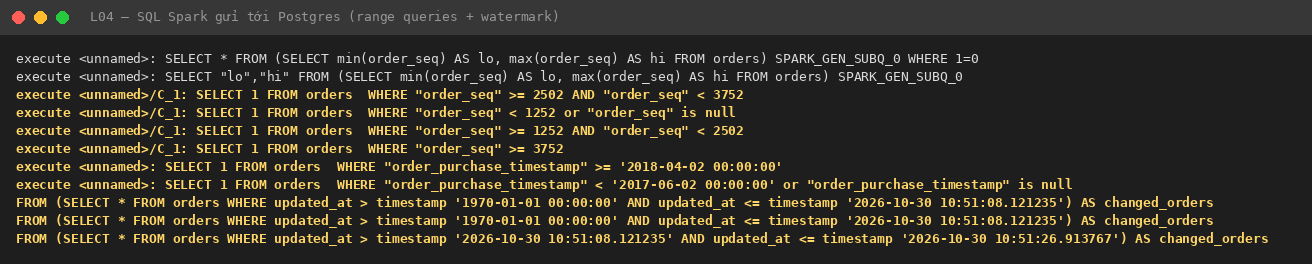
\includegraphics[width=1\linewidth,height=\textheight,keepaspectratio]{img/08_postgres_log_spark_sql.png}
\caption{Nhật ký PostgreSQL ghi lại các câu
\texttt{SELECT\ 1\ FROM\ orders\ WHERE\ .}\allowbreak{}\texttt{.}\allowbreak{}\texttt{.}\allowbreak{}
theo khoảng do Spark sinh ra.}\label{fig:l04-pglog-spark}
\end{figure}

Ghi Parquet với
\texttt{partitionBy("purchase\_}\allowbreak{}\texttt{month")}\allowbreak{}
mất 3.10 s, tạo 21 thư mục tháng (20 tháng lịch sử và tháng của các đơn
mới) chứa đủ 5,003 dòng. Truy vấn lọc
\texttt{purchase\_}\allowbreak{}\texttt{month\ =}\allowbreak{}\texttt{\ \textquotesingle{}2018-08\textquotesingle{}}\allowbreak{}
có physical plan chứa
\texttt{PartitionFilters:}\allowbreak{}\texttt{\ {[}isnotnull(purchase\_}\allowbreak{}\texttt{month\#118),}\allowbreak{}\texttt{\ (purchase\_}\allowbreak{}\texttt{month\#118\ =}\allowbreak{}\texttt{\ 2018-08){]}}\allowbreak{},
tức partition pruning có tác dụng. Năm bảng còn lại được nạp mỗi bảng
một partition (Bảng~\ref{tbl:l04-other}). Cả
\texttt{spark-submit\ -\/-step\ full}\allowbreak{} mất 21.2 s
(Hình~\ref{fig:l04-spark-full}).

\begin{longtable}[]{@{}ll@{}}
\caption{\label{tbl:l04-other}Số dòng các bảng phụ được Spark nạp sang
Parquet.}\tabularnewline
\toprule\noalign{}
Bảng & Số dòng \\
\midrule\noalign{}
\endfirsthead
\toprule\noalign{}
Bảng & Số dòng \\
\midrule\noalign{}
\endhead
\bottomrule\noalign{}
\endlastfoot
customers & 5,003 \\
order\_items & 5,852 \\
order\_payments & 5,472 \\
products & 1,500 \\
sellers & 312 \\
\end{longtable}

\begin{figure}
\centering
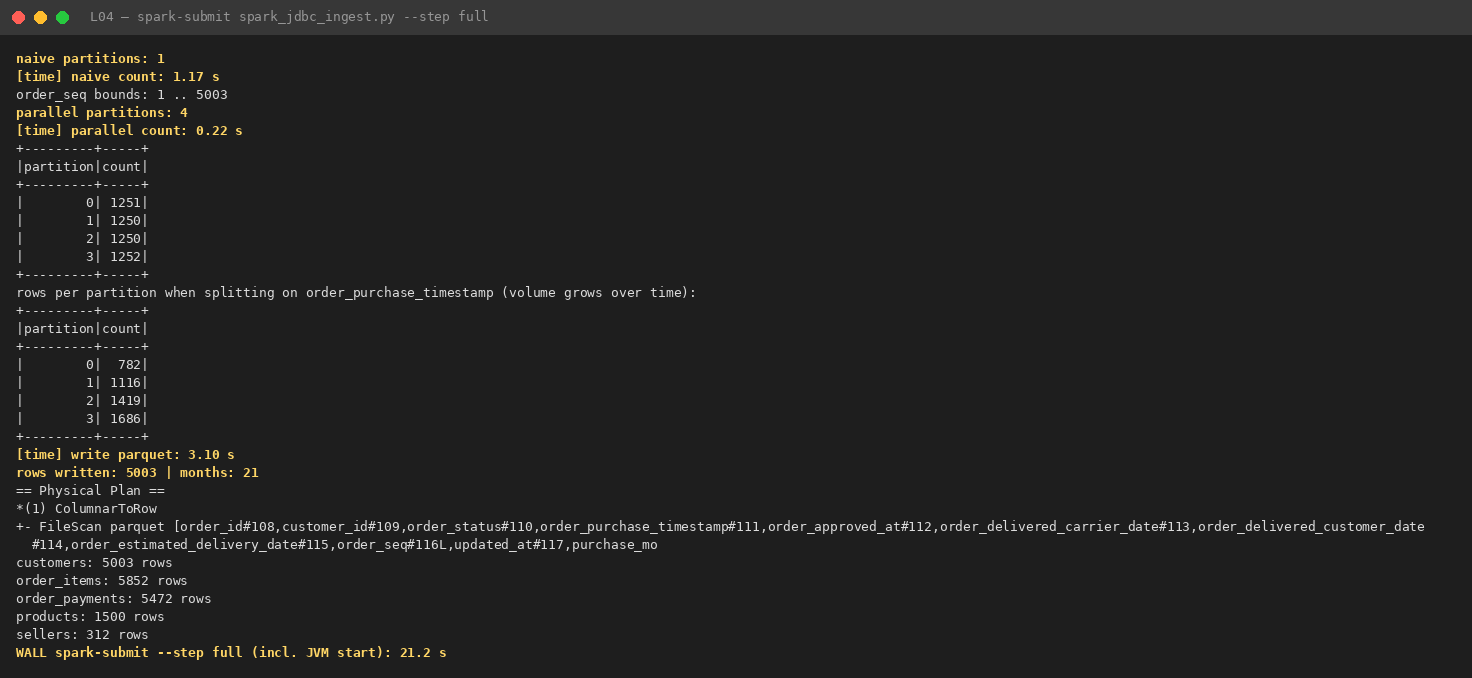
\includegraphics[width=0.85\linewidth,height=\textheight,keepaspectratio]{img/07_spark_full.png}
\caption{Kết quả \texttt{spark-submit\ -\/-step\ full}\allowbreak{}, gồm
physical plan có
\texttt{PartitionFilters}\allowbreak{}.}\label{fig:l04-spark-full}
\end{figure}

Trên Spark UI, các stage đọc song song và stage ghi Parquet đều có 4/4
task, đầu ra 680.4 KiB (Hình~\ref{fig:l04-spark-jobs},
Hình~\ref{fig:l04-spark-stages}). Trên HDFS,
\texttt{/}\allowbreak{}\texttt{data/}\allowbreak{}\texttt{olist/}\allowbreak{}\texttt{spark/}\allowbreak{}\texttt{orders}\allowbreak{}
có 22 mục (\texttt{\_SUCCESS} và 21 thư mục \texttt{purchase\_month=}),
dung lượng 680.4 K, còn
\texttt{/}\allowbreak{}\texttt{data/}\allowbreak{}\texttt{olist/}\allowbreak{}\texttt{sqoop/}\allowbreak{}\texttt{orders\_}\allowbreak{}\texttt{full}\allowbreak{}
là 1.0 M (Hình~\ref{fig:l04-hdfs}).

\begin{figure}
\centering
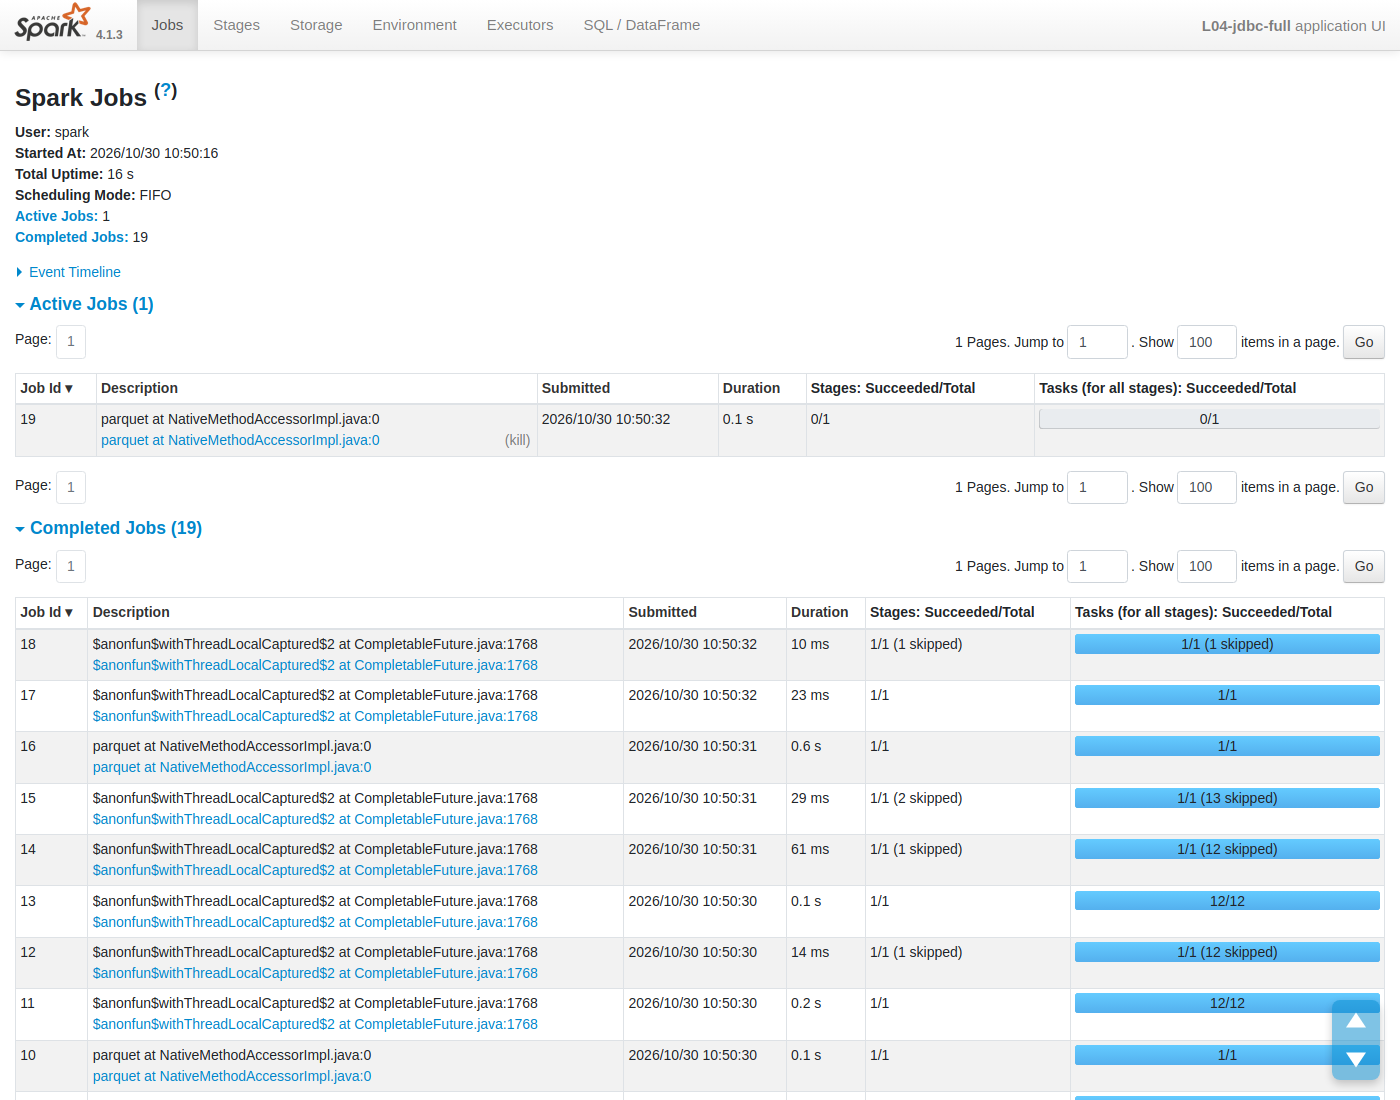
\includegraphics[width=1\linewidth,height=\textheight,keepaspectratio]{img/22_ui_spark_full_jobs.png}
\caption{Spark UI, trang Jobs của ứng dụng
\texttt{L04-jdbc-full}.}\label{fig:l04-spark-jobs}
\end{figure}

\begin{figure}
\centering
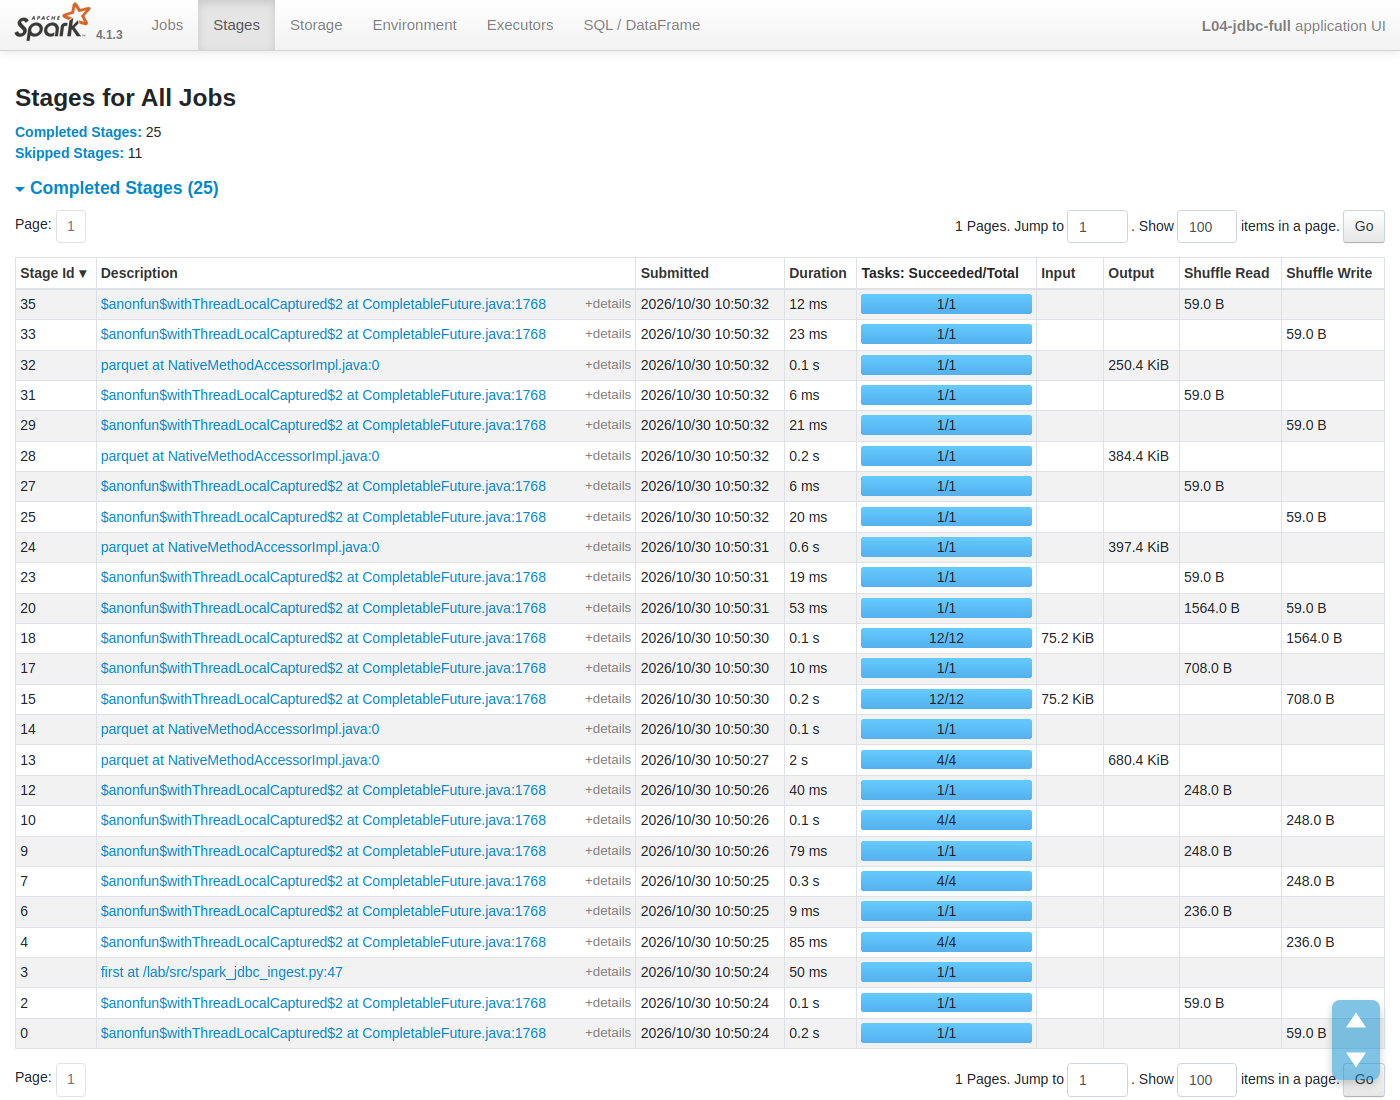
\includegraphics[width=1\linewidth,height=\textheight,keepaspectratio]{img/23_ui_spark_full_stages_4tasks.png}
\caption{Spark UI, trang Stages: các stage đọc JDBC song song và stage
ghi Parquet đều có 4 task.}\label{fig:l04-spark-stages}
\end{figure}

\begin{figure}
\centering
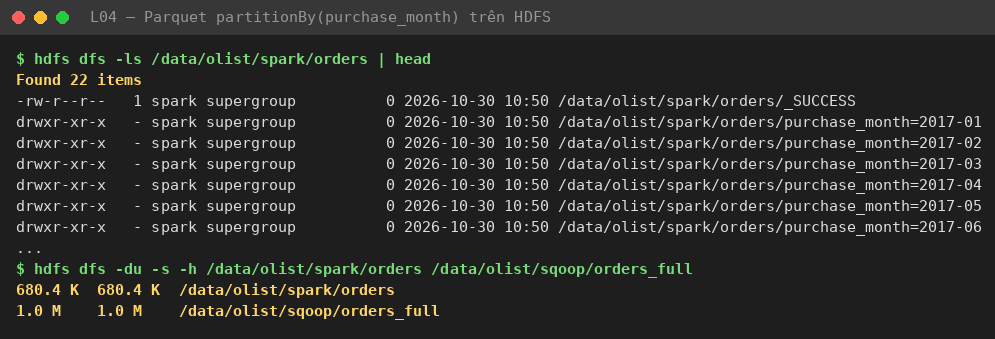
\includegraphics[width=0.85\linewidth,height=\textheight,keepaspectratio]{img/09_spark_output_hdfs.png}
\caption{Đầu ra Parquet phân vùng theo tháng trên HDFS và so sánh dung
lượng với đầu ra văn bản của Sqoop.}\label{fig:l04-hdfs}
\end{figure}

\subsection{Spark nạp gia tăng bằng watermark}\label{sec:l04-spark-incr}

Bước \texttt{incremental} chốt cận trên bằng \texttt{now()} của cơ sở dữ
liệu trước khi đọc, đọc cửa sổ
\texttt{(wm\_}\allowbreak{}\texttt{old,}\allowbreak{}\texttt{\ wm\_}\allowbreak{}\texttt{new{]}}\allowbreak{}
theo \texttt{updated\_at}, nối vào change log \texttt{orders\_changes},
dựng snapshot \texttt{orders\_current} bằng \texttt{row\_number()} theo
\texttt{order\_id} (sắp
\texttt{updated\_}\allowbreak{}\texttt{at\ DESC,}\allowbreak{}\texttt{\ \_}\allowbreak{}\texttt{ingested\_}\allowbreak{}\texttt{at\ DESC}\allowbreak{}),
và chỉ ghi watermark sau cùng:

\begin{Shaded}
\begin{Highlighting}[]
\NormalTok{wm\_new }\OperatorTok{=}\NormalTok{ jdbc(spark, query}\OperatorTok{=}\StringTok{"SELECT to\_char(now(), \textquotesingle{}YYYY{-}MM{-}DD HH24:MI:SS.US\textquotesingle{}) AS ts"}\NormalTok{).first().ts}
\NormalTok{changed\_sql }\OperatorTok{=}\NormalTok{ (}\SpecialStringTok{f"(SELECT * FROM orders WHERE updated\_at \textgreater{} timestamp \textquotesingle{}}\SpecialCharTok{\{}\NormalTok{wm\_old}\SpecialCharTok{\}}\SpecialStringTok{\textquotesingle{}"}
               \SpecialStringTok{f" AND updated\_at \textless{}= timestamp \textquotesingle{}}\SpecialCharTok{\{}\NormalTok{wm\_new}\SpecialCharTok{\}}\SpecialStringTok{\textquotesingle{}) AS changed\_orders"}\NormalTok{)}
\CommentTok{\# ... ghi changes (kèm cột \_ingested\_at) vào orders\_changes, rồi dựng snapshot:}
\NormalTok{log }\OperatorTok{=}\NormalTok{ spark.read.parquet(}\SpecialStringTok{f"}\SpecialCharTok{\{}\NormalTok{BASE}\SpecialCharTok{\}}\SpecialStringTok{/orders\_changes"}\NormalTok{)}
\NormalTok{w }\OperatorTok{=}\NormalTok{ Window.partitionBy(}\StringTok{"order\_id"}\NormalTok{) }\OperatorTok{\textbackslash{}}
\NormalTok{    .orderBy(F.col(}\StringTok{"updated\_at"}\NormalTok{).desc(), F.col(}\StringTok{"\_ingested\_at"}\NormalTok{).desc())}
\NormalTok{current }\OperatorTok{=}\NormalTok{ log.withColumn(}\StringTok{"\_rn"}\NormalTok{, F.row\_number().over(w)).}\BuiltInTok{filter}\NormalTok{(}\StringTok{"\_rn = 1"}\NormalTok{).drop(}\StringTok{"\_rn"}\NormalTok{)}
\NormalTok{current.write.mode(}\StringTok{"overwrite"}\NormalTok{).parquet(}\SpecialStringTok{f"}\SpecialCharTok{\{}\NormalTok{BASE}\SpecialCharTok{\}}\SpecialStringTok{/orders\_current"}\NormalTok{)}
\NormalTok{spark.createDataFrame([(wm\_new,)], }\StringTok{"watermark string"}\NormalTok{).coalesce(}\DecValTok{1}\NormalTok{) }\OperatorTok{\textbackslash{}}
\NormalTok{    .write.mode(}\StringTok{"overwrite"}\NormalTok{).json(}\SpecialStringTok{f"}\SpecialCharTok{\{}\NormalTok{BASE}\SpecialCharTok{\}}\SpecialStringTok{/\_state/orders\_watermark"}\NormalTok{)}
\end{Highlighting}
\end{Shaded}

Kết quả ba lần chạy ở Bảng~\ref{tbl:l04-spark-incr} và
Hình~\ref{fig:l04-spark-incr}.

\begin{longtable}[]{@{}
  >{\raggedright\arraybackslash}p{(\linewidth - 8\tabcolsep) * \real{0.2000}}
  >{\raggedright\arraybackslash}p{(\linewidth - 8\tabcolsep) * \real{0.2000}}
  >{\raggedright\arraybackslash}p{(\linewidth - 8\tabcolsep) * \real{0.2000}}
  >{\raggedright\arraybackslash}p{(\linewidth - 8\tabcolsep) * \real{0.2000}}
  >{\raggedright\arraybackslash}p{(\linewidth - 8\tabcolsep) * \real{0.2000}}@{}}
\caption{\label{tbl:l04-spark-incr}Kết quả ba lần chạy Spark nạp gia
tăng (thời điểm ngày 2026-10-30).}\tabularnewline
\toprule\noalign{}
\begin{minipage}[b]{\linewidth}\raggedright
Lần chạy
\end{minipage} & \begin{minipage}[b]{\linewidth}\raggedright
Cửa sổ watermark
\end{minipage} & \begin{minipage}[b]{\linewidth}\raggedright
Dòng đọc được
\end{minipage} & \begin{minipage}[b]{\linewidth}\raggedright
Change log
\end{minipage} & \begin{minipage}[b]{\linewidth}\raggedright
Snapshot
\end{minipage} \\
\midrule\noalign{}
\endfirsthead
\toprule\noalign{}
\begin{minipage}[b]{\linewidth}\raggedright
Lần chạy
\end{minipage} & \begin{minipage}[b]{\linewidth}\raggedright
Cửa sổ watermark
\end{minipage} & \begin{minipage}[b]{\linewidth}\raggedright
Dòng đọc được
\end{minipage} & \begin{minipage}[b]{\linewidth}\raggedright
Change log
\end{minipage} & \begin{minipage}[b]{\linewidth}\raggedright
Snapshot
\end{minipage} \\
\midrule\noalign{}
\endhead
\bottomrule\noalign{}
\endlastfoot
1 (chưa có watermark) &
\texttt{(1970-01-01\ 00:}\allowbreak{}\texttt{00:}\allowbreak{}\texttt{00,}\allowbreak{}\texttt{\ 2026-10-30\ 10:}\allowbreak{}\texttt{51:}\allowbreak{}\texttt{08.}\allowbreak{}\texttt{121235{]}}\allowbreak{}
& 5,003 & 5,003 & 5,003 \\
\texttt{simulate\_}\allowbreak{}\texttt{changes}\allowbreak{} lần 2 &
tạo 5004--5006, cập nhật đơn 337 và 355 & & & \\
2 &
\texttt{(10:}\allowbreak{}\texttt{51:}\allowbreak{}\texttt{08.}\allowbreak{}\texttt{121235,}\allowbreak{}\texttt{\ 10:}\allowbreak{}\texttt{51:}\allowbreak{}\texttt{26.}\allowbreak{}\texttt{913767{]}}\allowbreak{}
& \textbf{5} & 5,008 & 5,006 \\
3 (không có thay đổi) &
\texttt{(10:}\allowbreak{}\texttt{51:}\allowbreak{}\texttt{26.}\allowbreak{}\texttt{913767,}\allowbreak{}\texttt{\ 10:}\allowbreak{}\texttt{51:}\allowbreak{}\texttt{44.}\allowbreak{}\texttt{317579{]}}\allowbreak{}
& 0 & 5,008 & 5,006 \\
\end{longtable}

Change log giữ mọi phiên bản (\(5003 + 5 = 5008\)), còn snapshot chỉ giữ
phiên bản mới nhất của mỗi đơn (\(5003 + 3 = 5006\)), nên hai đơn được
cập nhật không bị nhân đôi. Lần thứ ba đọc 0 dòng: watermark được lưu
đúng và chạy lại không làm sai kết quả. Cận trên của lần trước trùng
khít với cận dưới của lần sau.

\begin{figure}
\centering
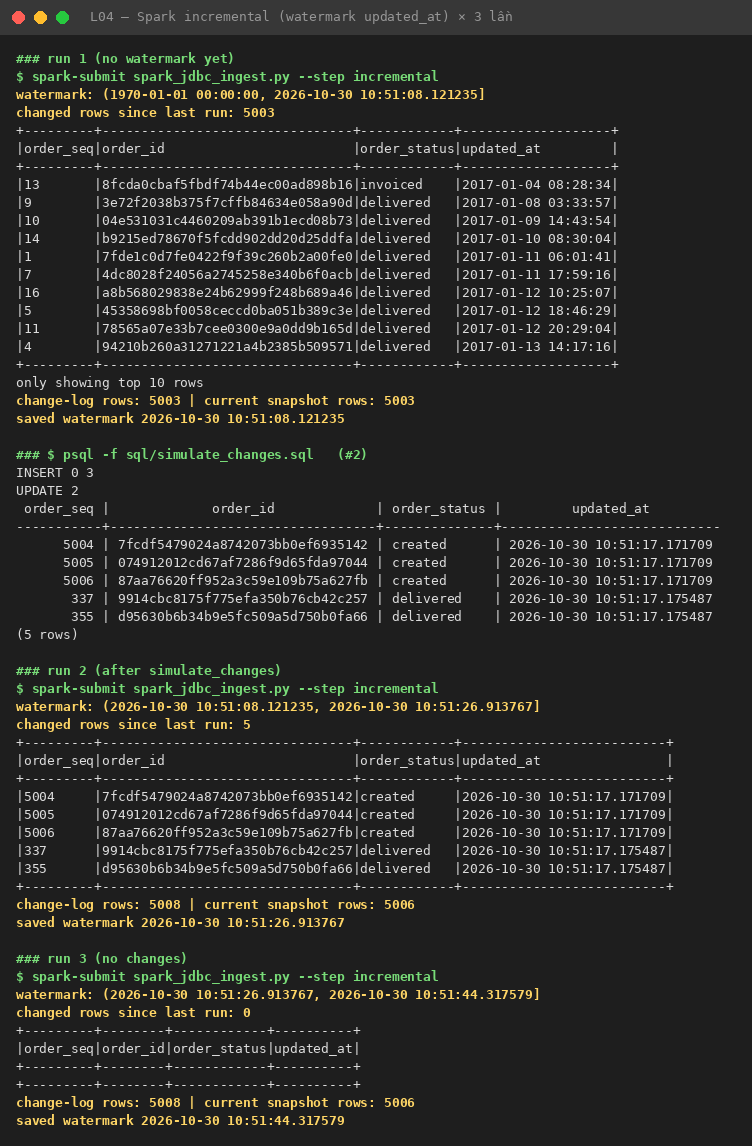
\includegraphics[width=0.85\linewidth,height=\textheight,keepaspectratio]{img/10_spark_incremental_3runs.png}
\caption{Ba lần chạy Spark
\texttt{-\/-step\ incremental}\allowbreak{}.}\label{fig:l04-spark-incr}
\end{figure}

\subsection{So sánh Sqoop và Spark JDBC}\label{sec:l04-compare}

Bảng so sánh của Phần 3 trong đề, kèm thời gian đo được, nằm ở
Bảng~\ref{tbl:l04-compare}.

\begin{longtable}[]{@{}
  >{\raggedright\arraybackslash}p{(\linewidth - 4\tabcolsep) * \real{0.3333}}
  >{\raggedright\arraybackslash}p{(\linewidth - 4\tabcolsep) * \real{0.3333}}
  >{\raggedright\arraybackslash}p{(\linewidth - 4\tabcolsep) * \real{0.3333}}@{}}
\caption{\label{tbl:l04-compare}So sánh Sqoop và Spark JDBC khi nạp bảng
\texttt{orders}.}\tabularnewline
\toprule\noalign{}
\begin{minipage}[b]{\linewidth}\raggedright
Tiêu chí
\end{minipage} & \begin{minipage}[b]{\linewidth}\raggedright
Sqoop 1.4.7 (MapReduce)
\end{minipage} & \begin{minipage}[b]{\linewidth}\raggedright
Spark JDBC
\end{minipage} \\
\midrule\noalign{}
\endfirsthead
\toprule\noalign{}
\begin{minipage}[b]{\linewidth}\raggedright
Tiêu chí
\end{minipage} & \begin{minipage}[b]{\linewidth}\raggedright
Sqoop 1.4.7 (MapReduce)
\end{minipage} & \begin{minipage}[b]{\linewidth}\raggedright
Spark JDBC
\end{minipage} \\
\midrule\noalign{}
\endhead
\bottomrule\noalign{}
\endlastfoot
Tham số song song & \texttt{-m\ 4} + \texttt{-\/-split-by} &
\texttt{numPartitions=4} + \texttt{partitionColumn} \\
Cách tính khoảng & Sqoop tự chạy \texttt{SELECT\ MIN,\ MAX}
(BoundingValsQuery) & người dùng truyền
\texttt{lowerBound}/\texttt{upperBound} (chỉ là stride) \\
Nạp gia tăng & Có sẵn:
\texttt{-\/-incremental\ append/}\allowbreak{}\texttt{lastmodified}\allowbreak{},
saved job lưu last value & Tự viết: truy vấn watermark + file trạng
thái \\
Xử lý UPDATE & \texttt{-\/-merge-key} (thêm một MR job) &
\texttt{row\_number()} khử trùng lặp, hoặc MERGE vào table format \\
Định dạng đầu ra & Văn bản CSV, 1.0 MB & Parquet Snappy phân vùng theo
tháng, 680.4 KB \\
Biến đổi khi nạp & Không (chỉ SQL qua \texttt{-\/-query}) & Đầy đủ
DataFrame API (\texttt{withColumn}, \texttt{partitionBy}, \ldots) \\
Thời gian nạp \texttt{orders} & 25.2 s MR job (28.5 s cả lệnh) & 3.10 s
ghi Parquet (21.2 s cả \texttt{spark-submit} 6 bảng, gồm khởi động
JVM) \\
Trạng thái dự án & Apache Attic (ngừng từ 2021) & Đang phát triển \\
\end{longtable}

Sqoop chậm chủ yếu vì mỗi lệnh phải sinh mã, biên dịch lớp record và
dựng một MapReduce job riêng. Spark dùng một SparkSession cho cả 6 bảng
và ghi thẳng ra định dạng cột có nén, nên đầu ra nhỏ hơn khoảng một phần
ba. Tuy vậy mọi thứ chạy trên một máy với khoảng 1 MB dữ liệu, thời gian
đo phản ánh chi phí khởi động nhiều hơn thông lượng, nên chênh lệch thời
gian chỉ nên hiểu theo nghĩa định tính.

\section{Trả lời câu hỏi checkpoint}\label{sec:l04-discussion}

\subsection{Sqoop chạy câu SQL nào trước khi import, và từ đó ra 4 split
bằng cách nào?}\label{sec:l04-q1}

Sqoop chạy bounding query
\texttt{SELECT\ MIN("order\_}\allowbreak{}\texttt{seq"),}\allowbreak{}\texttt{\ MAX("order\_}\allowbreak{}\texttt{seq")\ FROM\ "orders"}\allowbreak{}
và nhận (1, 5000) (Hình~\ref{fig:l04-pglog-sqoop}). Bộ chia số nguyên
cắt đoạn này thành 4 khoảng bằng nhau về giá trị, rộng khoảng
\((5000-1)/4 \approx 1250\); mỗi map chạy
\texttt{WHERE\ order\_}\allowbreak{}\texttt{seq\ \textgreater{}=}\allowbreak{}\texttt{\ lo\ AND\ order\_}\allowbreak{}\texttt{seq\ \textless{}\ hi}\allowbreak{},
khoảng cuối dùng \texttt{\textless{}=} để lấy cả MAX
(Bảng~\ref{tbl:l04-sqoop-splits}). Vì chia theo giá trị chứ không theo
số dòng, các split chỉ đều khi cột chia phân bố đều.

\subsection{\texorpdfstring{Vì sao các file \texttt{customers} không
đều, và nếu dùng
\texttt{-\/-split-by\ customer\_}\allowbreak{}\texttt{id}\allowbreak{}
thì
sao?}{Vì sao các file customers không đều, và nếu dùng -\/-split-by customer\_id thì sao?}}\label{sec:l04-q2}

Sqoop chia đều theo giá trị, nhưng zip code của khách hàng Olist dồn về
São Paulo, nên khoảng đầu {[}1014, 24536) nhận gần nửa bảng còn khoảng
{[}48057, 71578) rất ít (Bảng~\ref{tbl:l04-skew},
Bảng~\ref{tbl:l04-bucket}). Đây là data skew: task nặng nhất quyết định
thời gian của cả job. Còn \texttt{customer\_id} là chuỗi hash kiểu text;
mặc định Sqoop từ chối chia theo cột text và báo lỗi, trừ khi bật
\texttt{-Dorg.}\allowbreak{}\texttt{apache.}\allowbreak{}\texttt{sqoop.}\allowbreak{}\texttt{splitter.}\allowbreak{}\texttt{allow\_}\allowbreak{}\texttt{text\_}\allowbreak{}\texttt{splitter=}\allowbreak{}\texttt{true}\allowbreak{}.
Kể cả khi bật, việc chia theo thứ tự chuỗi phụ thuộc collation nên split
vẫn có thể lệch hoặc rỗng. Cột chia tốt nhất là cột số, phân bố đều và
có chỉ mục, như \texttt{order\_seq}.

\subsection{\texorpdfstring{Với
\texttt{lowerBound=}\allowbreak{}\texttt{1,}\allowbreak{}\texttt{\ upperBound=}\allowbreak{}\texttt{5003,}\allowbreak{}\texttt{\ numPartitions=}\allowbreak{}\texttt{4}\allowbreak{},
Spark có đọc dòng \texttt{order\_seq} = 9,999
không?}{Với lowerBound=1, upperBound=5003, numPartitions=4, Spark có đọc dòng order\_seq = 9,999 không?}}\label{sec:l04-q3}

Có đọc. \texttt{lowerBound} và \texttt{upperBound} chỉ dùng để tính bước
chia, không phải bộ lọc: partition cuối là
\texttt{order\_}\allowbreak{}\texttt{seq\ \textgreater{}=}\allowbreak{}\texttt{\ 3752}\allowbreak{}
không có cận trên (Hình~\ref{fig:l04-pglog-spark}), nên dòng 9,999 rơi
vào partition cuối; giá trị nhỏ hơn \texttt{lowerBound} và NULL rơi vào
partition đầu. Cận sai không làm mất dữ liệu, nhưng partition hai đầu sẽ
phình to và gây skew. Vì vậy script lấy MIN/MAX thật trước khi đọc, nhờ
đó 4 partition gần đều (Bảng~\ref{tbl:l04-spark-read}).

\subsection{Vì sao phải chốt cận trên trước khi đọc, và chỉ lưu
watermark sau khi ghi xong?}\label{sec:l04-q4}

Script lấy \texttt{wm\_new\ =\ now()} trước khi đọc, rồi truy vấn
\texttt{updated\_}\allowbreak{}\texttt{at\ \textgreater{}\ wm\_}\allowbreak{}\texttt{old\ AND\ updated\_}\allowbreak{}\texttt{at\ \textless{}=}\allowbreak{}\texttt{\ wm\_}\allowbreak{}\texttt{new}\allowbreak{}
(Mục~\ref{sec:l04-spark-incr}). Nếu lấy \texttt{now()} sau khi đọc, dòng
được cập nhật trong lúc đang đọc sẽ có \texttt{updated\_at} nhỏ hơn
watermark mới mà không nằm trong dữ liệu vừa đọc, và lần sau bị bỏ qua
luôn. Cận trên cố định còn bảo đảm các partition JDBC song song cùng
nhìn một cửa sổ, và các cửa sổ liên tiếp liền nhau mà không chồng lên
nhau, đúng như cận của ba lần chạy ở Bảng~\ref{tbl:l04-spark-incr}.

Về thứ tự lưu, nếu job chết giữa chừng thì watermark cũ vẫn còn và lần
chạy lại đọc lại cả cửa sổ. Dữ liệu có thể trùng nhưng không mất
(\emph{at-least-once}), và phần trùng được loại bằng
\texttt{row\_number()} khi dựng snapshot. Ngược lại, nếu lưu watermark
trước rồi bước ghi thất bại, cửa sổ đó sẽ không bao giờ được đọc lại.

\subsection{\texorpdfstring{Chế độ \texttt{append} hay
\texttt{lastmodified} bắt được UPDATE, và chế độ nào bắt được
DELETE?}{Chế độ append hay lastmodified bắt được UPDATE, và chế độ nào bắt được DELETE?}}\label{sec:l04-q5}

\texttt{append} chỉ dựa vào
\texttt{order\_}\allowbreak{}\texttt{seq\ \textgreater{}\ last\_}\allowbreak{}\texttt{value}\allowbreak{}
nên chỉ bắt được INSERT: saved job chỉ lấy các đơn mới
(Bảng~\ref{tbl:l04-sqoop-incr}). \texttt{lastmodified} dựa vào
\texttt{updated\_at} nên bắt được cả INSERT và UPDATE (thêm đơn 139 và
278); khi đó cần \texttt{-\/-merge-key} để gộp bản cũ với bản mới. Không
chế độ nào bắt được DELETE, vì dòng đã xóa không còn trong bảng để truy
vấn.

\subsection{\texorpdfstring{Watermark trên \texttt{updated\_at} không
giải quyết được gì, và CDC khác ở
đâu?}{Watermark trên updated\_at không giải quyết được gì, và CDC khác ở đâu?}}\label{sec:l04-q6}

Thứ nhất là DELETE: dòng bị xóa không bao giờ xuất hiện trong truy vấn,
nên bản sao trên HDFS giữ lại dữ liệu đã không còn ở nguồn, trừ khi ứng
dụng dùng soft delete hoặc so sánh cả snapshot. Thứ hai là các lần
UPDATE trung gian: nếu một đơn đổi từ \texttt{shipped} sang
\texttt{delivered} rồi \texttt{canceled} trong cùng một chu kỳ, chỉ
trạng thái cuối được thấy. Ngoài ra \texttt{updated\_at} có thể không
đáng tin: ứng dụng quên cập nhật cột, đồng hồ máy chủ lệch, hoặc một
transaction dài commit sau khi watermark đã vượt qua timestamp của nó và
dòng đó bị sót. Cách này cũng tạo tải quét lên nguồn (cần chỉ mục trên
\texttt{updated\_at}), và độ trễ bằng chu kỳ lập lịch.

CDC (Debezium, sẽ làm ở L08) không truy vấn bảng mà đọc write-ahead log
(WAL) của PostgreSQL qua logical decoding {[}3{]}, {[}4{]}. Mọi INSERT,
UPDATE và DELETE thành sự kiện theo thứ tự commit, kèm ảnh trước và sau,
không phụ thuộc \texttt{updated\_at}, gần như không tạo tải truy vấn và
trễ chỉ vài giây.

\subsection{\texorpdfstring{Điều gì xảy ra với cơ sở dữ liệu nguồn khi
đặt \texttt{-m\ 50} hoặc
\texttt{numPartitions=}\allowbreak{}\texttt{50}\allowbreak{}?}{Điều gì xảy ra với cơ sở dữ liệu nguồn khi đặt -m 50 hoặc numPartitions=50?}}\label{sec:l04-q7}

Nguồn nhận 50 kết nối đồng thời, mỗi kết nối một range scan. Con số này
dễ chạm \texttt{max\_connections} (PostgreSQL mặc định 100) khiến ứng
dụng production không lấy được kết nối, và các truy vấn tranh CPU, I/O,
buffer cache với tải OLTP; nếu cơ sở dữ liệu đã là nút thắt thì tốc độ
gần như không tăng. Với bảng 5,000 dòng, mỗi task chỉ còn khoảng 100
dòng, chi phí khởi tạo lớn hơn lợi ích. Thực tế nên giữ khoảng 4--8 kết
nối, thống nhất với DBA, đọc từ read replica hoặc ngoài giờ cao điểm.

\section{Kết luận}\label{sec:l04-conclusion}

Bài đã hoàn thành đủ phần Sqoop (nạp toàn phần, cột chia lệch,
\texttt{append}, saved job, \texttt{lastmodified} kèm merge, export),
phần Spark JDBC (đọc song song, Parquet phân vùng theo tháng, nạp gia
tăng bằng watermark) và bảng so sánh. Nhật ký SQL cho thấy cả hai công
cụ chia bảng theo khoảng giá trị, nên \texttt{order\_seq} cho các task
đều còn zip code và timestamp thì lệch. \texttt{append} chỉ bắt INSERT,
\texttt{lastmodified} và watermark bắt thêm UPDATE, còn DELETE và phiên
bản trung gian cần CDC.

\section*{Tài liệu tham khảo}\label{tuxe0i-liux1ec7u-tham-khux1ea3o}
\addcontentsline{toc}{section}{Tài liệu tham khảo}

{[}1{]} The Apache Software Foundation, ``Sqoop User Guide (v1.4.7),''
2017. https://sqoop.apache.org/docs/1.4.7/SqoopUserGuide.html

{[}2{]} The Apache Software Foundation, ``JDBC To Other Databases,''
Spark SQL Guide.
https://spark.apache.org/docs/latest/sql-data-sources-jdbc.html

{[}3{]} The PostgreSQL Global Development Group, ``Logical Decoding,''
PostgreSQL Documentation.
https://www.postgresql.org/docs/current/logicaldecoding.html

{[}4{]} Debezium Community, ``Debezium Connector for PostgreSQL,''
Debezium Documentation.
https://debezium.io/documentation/reference/stable/connectors/postgresql.html

\section*{Phụ lục: Tệp nộp
kèm}\label{phux1ee5-lux1ee5c-tux1ec7p-nux1ed9p-kuxe8m}
\addcontentsline{toc}{section}{Phụ lục: Tệp nộp kèm}

Đoạn mã tự viết chính đã trích trong Mục~\ref{sec:l04-spark-incr}; tệp
đầy đủ ở Bảng~\ref{tbl:l04-files}.

\begin{longtable}[]{@{}
  >{\raggedright\arraybackslash}p{(\linewidth - 2\tabcolsep) * \real{0.5000}}
  >{\raggedright\arraybackslash}p{(\linewidth - 2\tabcolsep) * \real{0.5000}}@{}}
\caption{\label{tbl:l04-files}Danh mục tệp nộp kèm báo cáo
L04.}\tabularnewline
\toprule\noalign{}
\begin{minipage}[b]{\linewidth}\raggedright
Tệp
\end{minipage} & \begin{minipage}[b]{\linewidth}\raggedright
Nội dung
\end{minipage} \\
\midrule\noalign{}
\endfirsthead
\toprule\noalign{}
\begin{minipage}[b]{\linewidth}\raggedright
Tệp
\end{minipage} & \begin{minipage}[b]{\linewidth}\raggedright
Nội dung
\end{minipage} \\
\midrule\noalign{}
\endhead
\bottomrule\noalign{}
\endlastfoot
\texttt{sqoop\_part1.sh},
\texttt{spark\_}\allowbreak{}\texttt{jdbc\_}\allowbreak{}\texttt{ingest.}\allowbreak{}\texttt{py}\allowbreak{}
& Lệnh Sqoop phần 1; script Spark JDBC đã hoàn thành \\
\texttt{01\_*.txt} đến \texttt{09\_*.txt}, \texttt{img/} & Log terminal,
nhật ký SQL của PostgreSQL, ảnh chụp terminal và UI \\
\end{longtable}

\end{document}
